%% Example TAMUCC MS Project
\documentclass{COSCMSproject}

%\usepackage[dvips]{graphicx,color}
\usepackage{amsfonts}
\usepackage{graphicx}
\usepackage{amsmath}
\usepackage{mathtools}
\usepackage{float}
\usepackage{tabularx}
\usepackage{array}
\usepackage{longtable}
\graphicspath{{image/}}
\providecommand{\abs}[1]{\lvert#1\rvert} 
\providecommand{\norm}[1]{\lVert#1\rVert}
\newcolumntype{C}[1]{>{\centering\let\newline\\\arraybackslash\hspace{0pt}}m{#1}}

%%%%%%%%%%%
% Type of document.
% Use the appropriate type.

\renewcommand{\type}{Project}   % Define this if proposal

\begin{document}
\pagenumbering{roman}

%%  Fill in the following information between the brackets
\newcommand{\thesistitle}{A Hybrid Data Mining Approach for Hyperspectral Images Analysis} %use \\Second Line of Title if needed
\newcommand{\authorsname}{Xinyi Wang}  % Author's Full Name	
\newcommand{\thesismonth}{Summer 2014}     % {Semester Year}
\newcommand{\committeechair}{Dr. Longzhuang Li}
\newcommand{\committeemembera}{Dr. Scott A. King}
 

% This will create the title and approval page, do not remove
%\maketitlepage
\approval

% Put the text of your abstract between the brackets
\theabstract{
Hyperspectral images are a series of image frames in different wavelength bands which form a cube of data with both spatial and spectral information. Data mining is to mine the useful data from the huge datasets. Since the pixels of hyperspectral images are all in very high dimensional space, data mining for hyperspectral images, or also called hyperspectral image classification, is quite challenging. A different approach with more process steps is introduced for better accuracy. The system contains hyperspectral data understanding, data preparation, vegetation detection algorithm, the k-means algorithm, and support vector machine. Data understanding is the first step to let people know about the datasets. Data preparation is the basic step for input of data mining algorithms because some of the algorithms need to have a specified format. Vegetation detection algorithm is to mine the useful data for the k-means algorithms. The k-means algorithm can generate some feature for support vector machine (SVM). SVM is to apply the features from the previous step and to mine the data, and finally some accuracies are generated according to those processes of hyperspectral imaging dataset, which helps us test the model.
}

\tableofcontents
\listoffigures     % If you have any
\listoftables     % If you have any
\clearpage
\pagenumbering{arabic}   % change from Roman back to Arabic

% the following parts of the project can go here in one big file or can
% be broken up into smaller files and included using the \include 
% for example have a file called ack.tex and use \include{ack}
% and another file called ch1.tex and use \include{ch1}
% Just like in software development breaking into smaller files has many
% advantages, however, you end up with a lot of extra files in your directory
% after latex and bibtex do their jobs.

%chapter1
\chapter{Introduction}
��Information age�� is a popular term to describe the world we are living in. However, what is information made up of? Actually it is a wide range of data. Data can be huge, but not all of them are useful for us. How do we abstract the useful data from it? A correct data mining technique is therefore important for numerous practical purposes, especially for the huge dataset. Data mining is currently being exploited in many applications, such as games, businesses and sciences. 

In this study, a hyperspectral imaging system is used to obtain the hyperspectral images of some mud from the Ocean. To mine the significant objects (such as algae) from these mud samples is the main purpose here. Finding the algae is good for environment protection, especially for coral protection. The general steps in this project are hyperspectral data understanding, pre-processing, unsupervised learning, feature selection, supervised learning (post-processing), and rules or decision. Data understanding is the first step to let people know about the datasets. Pre-processing is the basic step for data cleaning because the experimental datasets contain lots of noise or even missing data. Unsupervised learning is the next step to mine the data from the cleaned data by using K-means. Feature selection is the step right after unsupervised learning which can generate some feature after data mining algorithm. Supervised learning, also known as post-processing is to apply the features from the previous step and to mine the data, and finally some rules or decision is generated according to those processes of hyperspectral imaging dataset. These data mining algorithms are presented for hybrid techniques. The final goal of this paper is to test more data mining models for hyperspectral image data, including more processing in order to improve the accuracy, and finally provides some conclusions and recommendations regarding these methods.

\section{Statement of the Problem}
It is important for researchers to abstract the useful information from the huge dataset in any field. The question can be summarized as follows:

\textit{Given a dataset that contains information in the form of hyperspectral variables that are believed to significantly influence the objects, what are the most appropriate data mining techniques to determine useful information with a reasonable margin of error?}

To answer this question, this study explores several data mining methods that might be used to determine the significant objects by using data of hyperspectral images on mud samples. The main goal of this work focuses on studying the currently available applicable data mining tools (such as the k-means algorithm and support vector machine) for finding out the significant objects.

Hyperspectral image classification is the method used to abstract information from images. Finding the optimal approach for hyperspectral image classification for a given application becomes a popular research problem for computer scientists.

Hyperspectral images are a series of image frames in different wavelength bands which form a cube of data with both spatial and spectral information. In each pixel of the hyperspectral image, wavelength bands versus raw intensity counts (arbitrary units) can be obtained and graphed. Different objects have different spectral information in certain wavelength bands. Therefore, the goal is to understand the microdistribution of organisms, by analyzing the plots. Figure~\ref{fig11} gives you the idea of what a hyperspectral image look like.

\begin{figure}[H]
\centering
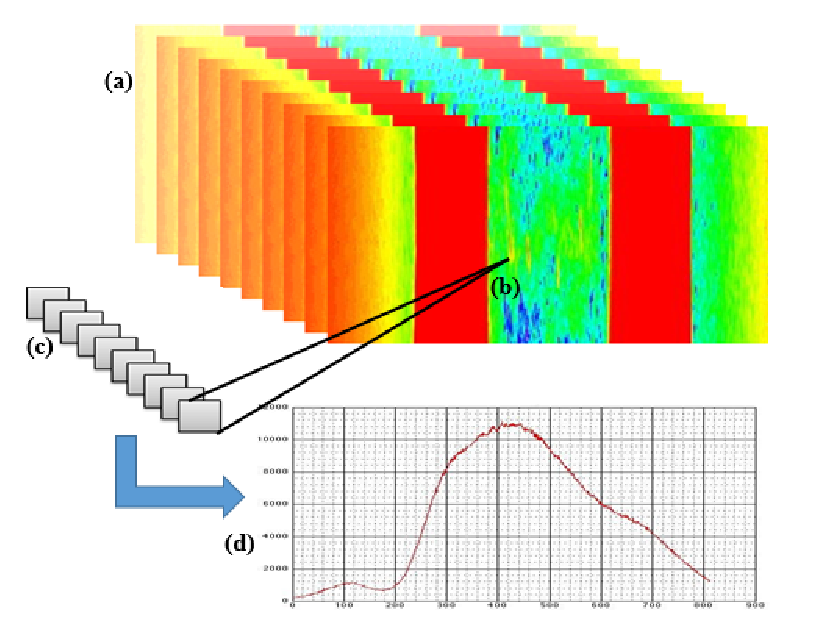
\includegraphics{fig11} 
\caption{
\label{fig11}  % use this to reference in text.
(a) A hyperspectral image of gold nanoparticles. (b) A single pixel location from the hyperspectral image. (c) The pixel at different frames with the same location. (d) The spectrum of the single pixel location, corresponding to a series of image frames at different wavelength.
}
\end{figure}

The essence of hyperspectral image classification using spectral analysis in this project involves processing data through data mining. Data mining refers to finding patterns in large data sets, such as the hyperspetral images, which can be as large as 20 Giga Bytes (GB) each.  Several algorithms have been defined in the data mining domain such as decision trees, artificial neural networks, K-means, and support vector machine (SVM) algorithm. Determining and building an efficient and accurate classifier based on the optimal data mining algorithm is one of the objectives of this mud hyperspectral image classification project.

In this study, the hybrid of pre-processing, unsupervised learning and supervised learning is presented for hyperspectral image analysis and surface classification from mud samples. In this system, the classifier has three layers: the first layer is for pre-processing. The medial layer is unsupervised learning, the k-means algorithm. The last layer represents supervised learning, support vector machine.

\section{Review of the Literature}
Since entering in the space age in 1957, people keep documenting the image data of Earth from outer space \cite{Lan2002}. The image information can be analyzed for different purposes, such as military uses, agriculture, and urban planning \cite{lili}. Hyperspectral images classification is more challenging because of the very high dimensionality of the pixels and the small number of labeled examples typically available for learning \cite{GVG}.

\subsection{Hyperspectral Image}
Because human eyes only can see the light under bands from 390nm to 750 nm, there are requirements for detecting visions, whose bands are below 390 nm or beyond 750nm \cite{SC}. For example, the gold nanoparticles are actually spherical organic coated particles, and dissolved in toluene. Then the gold nanoparticles dissolved in toluene were further diluted in different concentration of 14\%, 28\% and 50\% in toluene. Human eyes are mostly sensitive at around band of 555 nm.

\begin{figure}[H]
\centering
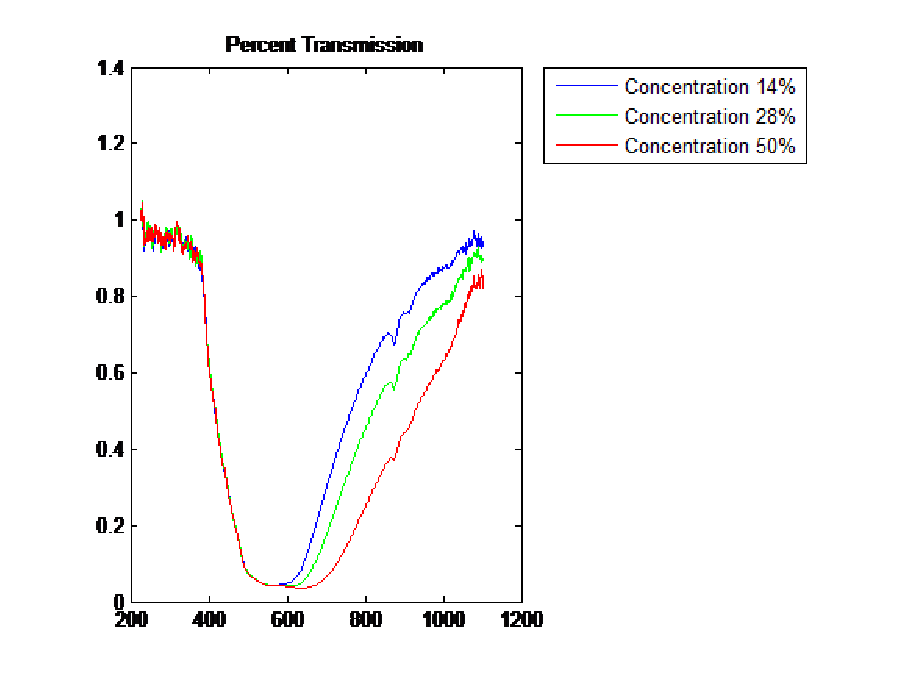
\includegraphics{fig12} 
\caption{
\label{fig12}  % use this to reference in text.
Percent Transmission of three different gold nanoparticle concentrations.}
\end{figure}

From Figure~\ref{fig12} mentioned, it shows that the figures of three samples overlap each other at around band of 555 nm but split up at band of 600 nm or above. It means that it is hard to identify the concentration of three samples by human eyes. If the research is extended beyond the visible, there are some significant differences between the samples.

\subsection{The Existing Approaches}
There are many existing approaches available for hyperspectral classification. The k-means algorithm and support vector machine are getting more attention because of the complexity of high dimensionality of hyperspectral images. Most of approaches are based on them with more process involved. A neighborhood-constrained k-means (NC-k-means) algorithm \cite{NCK} is developed to incorporate the pure neighborhood index into the traditional k-means algorithm. A parameter-free k-means algorithm \cite{KJE} is proposed in 2012, which is based on co-occurrence matrix scheme. Support vector machines for hyperspectral image classification with spectral-based kernels \cite{MGLM} are introduced in 2003. A support vector classification method for hyperspectral data based on spectral and morphological information is proposed in 2011 \cite{lili}. The semi-supervised classifier named PSO-SVM, which is combined by support vector machine (SVM) and particle swarm optimization (PSO), was proposed in 2010 \cite{GMGW}. They focus their results on either the accuracy or the running time, which means that they either get a better accuracy with a time-consuming system or reduce the running time to get a reasonable accuracy. Therefore, here comes our hybrid system with a reasonable accuracy and running time.

    

\section{Methodology}
Going back to the original research question: What data mining techniques can be used to find out the significant objects? The literature review in the previous section indicated different alternatives to answer this question. This study selects the techniques that were most successfully used in the literature. The real hyperspectral images of mud sample are used for solve the problem by using these different techniques and their results are compared.

A general data mining is used to find out the significant objects for mud samples. Chapter Two shows the technique of identifying how differences between the visible red and near-infrared bands of the mud sample image, which we can use this technique to identify the areas having the significant objects; k-means, a data mining technique, is an unsupervised learning, which means we can find out the classes or groups, and label them for the final data mining process, SVM; and the SVM technique that takes into account the classes or groups in training the unknown dataset, providing a prediction of each groups. Chapter Three shows how the approaches work and the system architecture. Chapter Four focuses on experimental results from testing a hyperspectral image. Finally, Chapter Five discusses these data mining techniques and provides conclusions and recommendations regarding these methods.

\section{The sample}
The hyperspectral image of the mud sample is taken from Hyperspectral Optical Property Instrumentation (HOPI) Lab at Texas A\&M University \textemdash Corpus Christi. Figure~\ref{fig14} shows the photo of the mud sample.

\begin{figure}[H]
\centering
\includegraphics{fig14} 
\caption{
\label{fig14}  % use this to reference in text.
The photo of the mud sample.}
\end{figure}

Figure~\ref{fig15} shows the hyperspectral image of the mud sample in MATLAB with gray scale and original axis.

\begin{figure}[H]
\centering
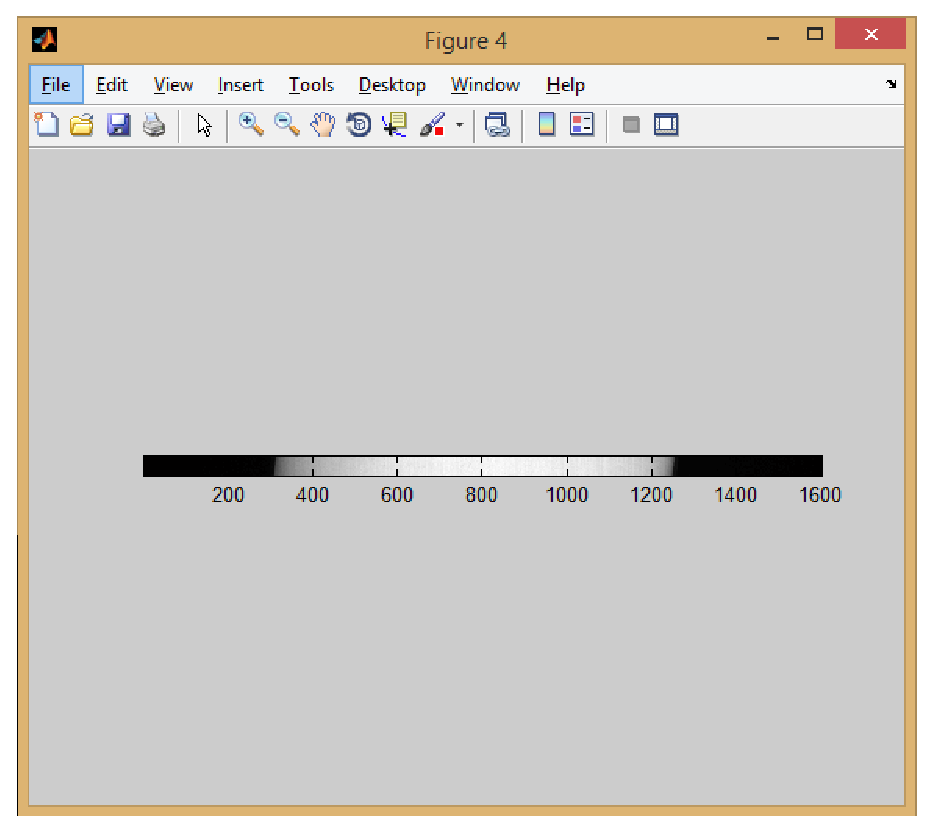
\includegraphics{fig15} 
\caption{
\label{fig15}  % use this to reference in text.
A hyperspectral image of a mud sample.}
\end{figure}

\section{Exploring the Dataset}
Each hyperspectral image has its own header file, which records the date of taking the image, samples, lines and bands. The important information is saved here for setting up the parameter when the image is processed. Figure~\ref{fig16} shows what the header file includes. The wavelength is continuously increased from 399.538849 nm to 999.494408 nm by 0.740686 nm.

\begin{figure}[H]
\centering
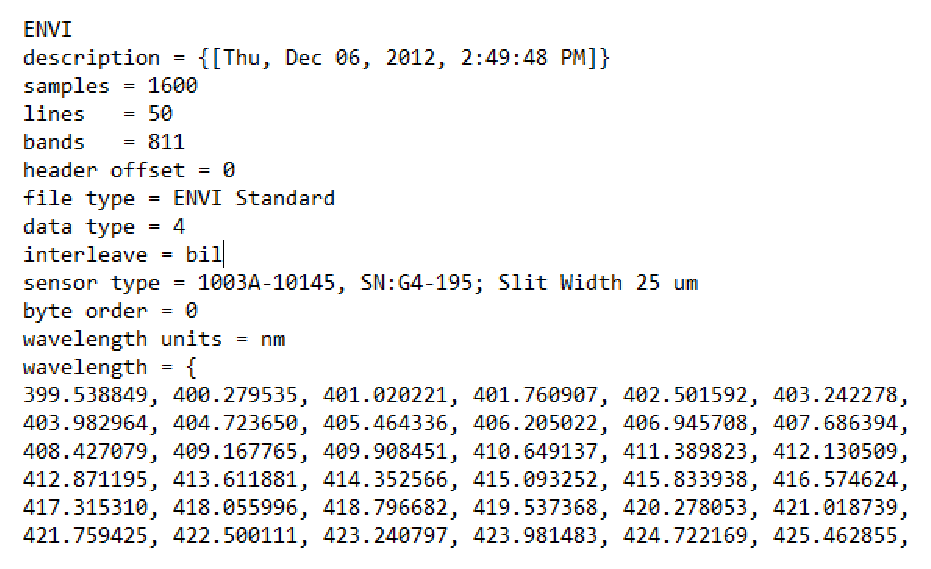
\includegraphics{fig16} 
\caption{
\label{fig16}  % use this to reference in text.
The header file of a hyperspectral image of a mud sample.}
\end{figure}

From Figure~\ref{fig15}, it shows that a hyperspectral image can be imported into MATLAB through the code below:

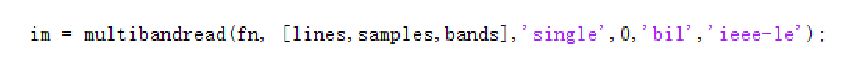
\includegraphics{code1} 

Once processed, the saved hyperspectral image is shown in the workspace of MATLAB:

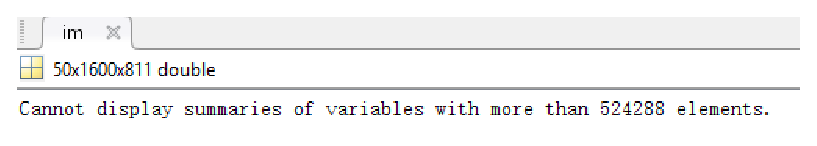
\includegraphics{code2} 

The size of the hyperspectral image of mud sample is 50-by-1600 with 811 bands in depth. Once the im is opened, it is said that:

\includegraphics{code3}

To process this hyperspectral image, data preparation in each chapter is always the first and important step to deal with. The Figure~\ref{fig17} is the hyerpsectral image of mud sample in MATLAB with color and square axis. Next, all the related algorithm or techniques is shown in Chapter Two.

\begin{figure}[H]
\centering
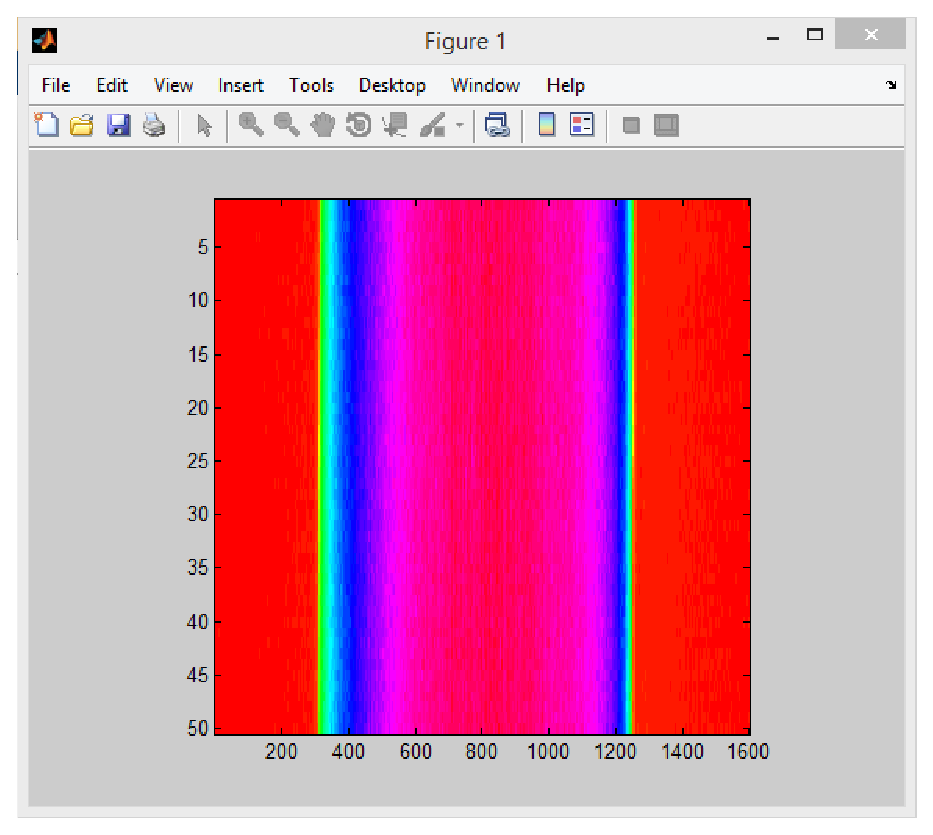
\includegraphics{fig17} 
\caption{
\label{fig17}  % use this to reference in text.
The hyperspectral image of mud sample in MATLAB with color and square axis.}
\end{figure}


%chapter2
\chapter{Related Work}
The related techniques or algorithms are vegetation detection algorithm, the k-means algorithm and support vector machine. Algorithm for vegetation detection can detect the hyperspectral image for the purpose of predicting the percentage of significant objects. The k-means algorithm, a centroid-based technique, will help us find out the clusters. The k-means algorithm is a cluster analysis algorithm, which mainly calculates data aggregation by constantly computing the average distances between each points and mean point. Machine learning is essentially an approximation of the true model of problems, which means the best approximate mode that is used for the true model is called a hypothesis. So there is no doubt that the true model is certainly unknown. Otherwise, the true model can just be used and there is no point to have machine learning. Since the true model is unknown, how much differences between the hypothesis and the real solution are also unknown. However, if some attributes or instances are known, they can be used to approach to the real model. Support Vector Machine is used to find the errors, approach the true model and predict the unknown model.


\section{The k-means algorithm for Hyperspectral Images}
The k-means algorithm is one of the major techniques to be used to classify the hyperspectral images. Several approaches related to the k-means algorithm are introduced for pursuing a better classification or a better accuracy.

A neighborhood-constrained k-means (NC-k-means) algorithm \cite{NCK} is developed to incorporate the pure neighborhood index into the traditional k-means algorithm. A neighbourhood is defined as a set of contiguous pixels in a certain window of an image. The size of a window is usually 2-by-2 pixels, 3-by-3 pixels, or 4-by-4 pixels. According to the definition of neighbourhood, a binary function called pure neighbourhood index (PNI) is defined by whether a neighbourhood is a pure neighbourhood of class k or a mixed neighbourhood of class k. The very first step is to classify the images into k clusters and initialize a set of centroids like the normal k-means algorithm does. Once the partition matrix is computed to classify all pixels to initial cluster k, the neighbourhood window scale can be set up. The next step is to calculate the spectral vector of each neighbourhood and determine the value of the neighbourhood label. Then PNI is used to calculate all neighbourhoods, and determine the total number of pixels in pure neighbourhoods. The final step is iteratively to calculate the k-means objective function and adjust the centroid of each cluster k, cluster type of each pixel and cluster type of each neighbourhood. This approach definitely reduce the interference of noise and the heterogeneity to have a better performance compared to the k-means algorithm. The NC-k-means algorithm with neighbourhood window size of 2-by-2 do not have the best results in any cases. The window size must be 3-by-3 or 4-by-4 to have a better performance in some cases. Therefore, the results of the NC-k-means algorithm is not always better than the k-means algorithm. 

A parameter-free k-means algorithm \cite{KJE} is proposed in 2012, which is based on co-occurrence matrix scheme. This method can be used to output the number of desired clusters. The input of this method is a dataset containing n objects. The process of the method is to transform the dataset images to gray scale images, and then transform them to co-occurrence matrix. The next step is to find out a diagonal matrix from the results of co-occurrence matrix. The final step is to determine the k value by finding out the number of local maximums. Since the number of clusters of this parameter-free method always has less than one of other algorithms, the algorithm is not sure to have enough precision. The running time of this method is not mentioned in the article, so it is hard to compare it with other methods.

\section{Support vector machine for Hyperspectral Images}
Due to the high dimensionality of the hyperspectral images, many data mining techniques can not have the reasonable performance. However, support vector machines (SVM) can still maintain a reasonable classification accuracy. 

Support vector machines for hyperspectral image classification with spectral-based kernels \cite{MGLM} are introduced. The difference between spectral kernels and usual kernels is that the spectral kernels are based on a quadratic distance evaluation between two samples. Spectral angle (SA) is defined to measure the spectral difference, and the spectral information divergence (SID) is also defined to measure the spectral difference with a different equation. Mixture between spectral-based and quadratic-based kernels is also developed to classify the images. However, the results are not given to us as an accuracy but a figure. It is really hard to confirm which kernel perform the best without the accuracies.

A support vector classification method for hyperspectral data based on spectral and morphological information is proposed in 2011 \cite{lili}. The very first step is to apply SVM-recursive feature elimination (RFE) to the original data to obtain the most discriminative spectral subset \begin{math}{S_i}\end{math}. The second step is to construct the extended multivariate morphological profile (EMMP) with the subset \begin{math}{S_i}\end{math} to obtain \begin{math}{EMMP_i}\end{math}. The third step is to apply nonparametric weighted feature extraction (NWFE) to the \begin{math}{EMMP_i}\end{math} to extract feature \begin{math}{MORP_i}\end{math}. The fourth step is to apply NWFE to the orightnal hyperspectral data to extract feature \begin{math}{SPEC_i}\end{math}. The next step is to fuse the \begin{math}{MORP_i}\end{math} and the \begin{math}{SPEC_i}\end{math} to obtain \begin{math}{MS_i}\end{math}. The final step is to use SVM classification based on the \begin{math}{MS_i}\end{math}. A feature selection algorithm can construct the EMMP more effectively. The classification accuracy is improved by the feature of the EMMP, but to construct the EMMP is very time-consuming.

A comparison of support vector machine, import vector machines and relevance vector machines for hyperspectral classification is proposed in 2011 \cite{BAC}. There are two of the proposed enhancements, import vector machines (IVM) and relevance vector machines (RVM), compared to the support vector machine. IVM is similar with SVM in the curve shape and the negative logarithmic likelihood of the binomial distribution. RVM is introduced as the Bayesian principle to the SVM concept. The dataset in this research is a small training data set and a large number of classes. Even though IVM and RVM outperform the SVM, the authors still say that more datasets should be involved to confirm the results.

The semi-supervised classifier named PSO-SVM, which is combined by support vector machine (SVM) and particle swarm optimization (PSO), was proposed in 2010 \cite{GMGW}. This approach inflates the unlabeled samples of hyperspectral images to obtain a result with higher accuracy. The particle estimates the parameter values and the candidates of the labels of the randomly selected unlabeled samples. The fitness function generated by PSO, is designed based on two concepts: the classification accuracy and the ratio calculated by the number of supported vectors divided by the number of samples. Most of the particles have a high accuracy classification. However, a small number of them with a low fitness value influence the result the most. First, find the candidate labels for the unlabeled samples trough a SVM trained by the labeled samples. Second, generate the particles from the unlabeled samples. Third, train SVM classifiers for each particles to inflate the samples. Fourth, apply the fitness function to particles. Fifth, classify the result with the test data. This approach has a better performance compared with other techniques. The RBF kernel function is only adopted in the SVM model, it is better to test with other kernel functions

\section{Discussion}
There are also other approaches to either achieve the goal of faster support vector classifications \cite{Fehr} or achieve the goal of improving the accuracy of support vector machine \cite{McCue}. The first approach to build up a SVM-tree and decompose the original problem into many linear subproblems with non-linear extensions. Every subproblem is treated as a linear case of SVM at first. If they think they have a good result of that subproblem in the linear case, they will not process anymore in non-linear case. Therefore, they do reduce the running time of processing the large dataset, but this definitely affects the accuracy. In the article, they also claim that they achieve just reasonable classification results. The second approach is about increasing the accuracy by tuning the parameters of support vector machine manually. Considering the average running time of SVM and k-means, finding out the appropriate parameters for SVM is more costly than finding out the appropriate clusters in k-means. Therefore, even though they improve the accuracy of SVM, the running time of SVM is more concerned if a large dataset is processed.
Therefore, a hybrid system is formed here to pursue a better accuracy with a reasonable running time. Algorithm for vegetation detection is the first step to detect percentage of significant objects of the hyperspectral image. The k-means algorithm, a centroid-based technique, is considered as the second step to help us identify the location of clusters. Support Vector Machine is used to be the last step to find the errors, approach the true model and provide the accuracy of this model.


%chapter3
\chapter{The Hybrid System Design}
Data preparation is the very first step of the algorithm. Figure~\ref{fig31} shows a diagram of the system architecture. The hyperspectral dataset is trained by using algorithm for vegetation detection, the k-means algorithm and support vector machine, and an unknown dataset is tested to get the accuracy by using the test mode, 10-fold cross-validation. 

\begin{figure}[H]
\includegraphics[width=\textwidth]{fig31} 
\caption{
\label{fig31}  % use this to reference in text.
The system architecture.}
\centering
\end{figure}

In this hybrid system, the number of clusters is not required as input because it can be predicted by the k-means algorithm. Using the k-means algorithm is relatively to reduce the running time of the entire system. The procedure of this hybrid system is data preparation for each algorithm; determine the percentage of the significant objects by using algorithm for vegetation detection; find out the clusters or groups of the hyperspectral image by using the k-means algorithm; and finally generate the training model and find out the accuracy by using support vector machine. Some experimental results are shown in the next chapter according to this system architecture. 

\section{Data Preparation}
The dataset is an 811-band 50-by-1600 hyperspectral image of a mud sample, whose pixel values are band interleaved by line (BIL) in order to increase band number. BIL is one of three primary methods for encoding multiband image data, which has the advantage of accessing the spatial and spectral data easily.

Since the hyperspectral image is a three dimensional dataset, it is not mathematically convenient to operate for the further data mining. Therefore, the three dimensional dataset is reformatted into two dimensional dataset by having each column display the entire pixel values of each layer or band, so we make a new 80000-by-811 dataset.

\section{Vegetation Detection Algorithm}
This algorithm tells us how to find out the differences between the visible red and near-infrared bands of a Landsat image and the percentage of the Vegetation. To predict the percentage, we need to find out the differences between the visible red and near-infrared bands of the hyperspectral image. This technique identifies the pixels or area that contains the significant objects, such as algae.

To achieve this result, there are six steps in this original algorithm \cite{Raj}, shown in Figure~\ref{alg1}:

\begin{figure}[H]
\centering

\includegraphics{alg1} 
\caption{
\label{alg1}  % use this to reference in text.
Vegetation detection algorithm.}
\end{figure}

The very first step is to select the three most informative bands from the mud sample file. To determine these three bands, we need to find out how many 0s are in each band. Therefore, by figuring out the three least 0s bands, we can know the three bands we want. With the three bands, we can continue to run our algorithm to find out the percentage of the significant objects.

The color-infrared (CIR) composite is the result when the near infrared (NIR), the visible red and the visible green are mapped into the red, green and blue planes of an RGB image. To read the hyperspectral image, the MATLAB function multibandread can help us handle it in a special form that we can recognize. Therefore, when we use the MATLAB function multibandread from the three determined bands, we have an RGB image, which red means the NIR band, green means the visible red band and blue means the visible green band. However, still the contrast is not as good as we want.

Next, we will construct an NIR-Red scatter plot, which helps us compare the NIR band (displayed as red) and the visible red band (displayed as green). As we said above, we can easily extract the NIR and red bands from the CIR composite. So we can see the difference between these two bands in grayscale images.

To find out the significant objects, we have to compute the index of each pixel:
\begin{equation} \text{Index = {(NIR - red) ./ (NIR + red)}} \end{equation}
In order to identify pixels most likely to contain significant objects, we apply a simple threshold to the image. We just need to create the significant objects image that have index greater than threshold. Percentage of significant objects is calculated by ratio of number of while pixels in binary image to total number of pixels in NIR image.

\section{The k-means Algorithm}
\subsection{Introduction}
A centroid-based partitioning technique uses the centroid of a cluster, \begin{math}C_i\end{math}, to represent that cluster. Conceptually, the centroid of a cluster is its center point. The centroid can be defined in various ways such as by the mean or medoid of the objects or points assigned to the cluster. The k-means algorithm is for partitioning, where each cluster\rq s center is represented by the mean value of the objects in the cluster \cite{HanJ}.

The k-means algorithm is a typical clustering algorithm based on distances, using distance as the similarity index for evaluation, which also considers the closer the objects, the greater the similarity. The clusters in this algorithm are determined by nearby objects, so the ultimate goal of this algorithm is to get compact and independent clusters. Figure~\ref{alg2} shows the k-means algorithm \cite{HanJ}.

\begin{figure}[H]
\centering
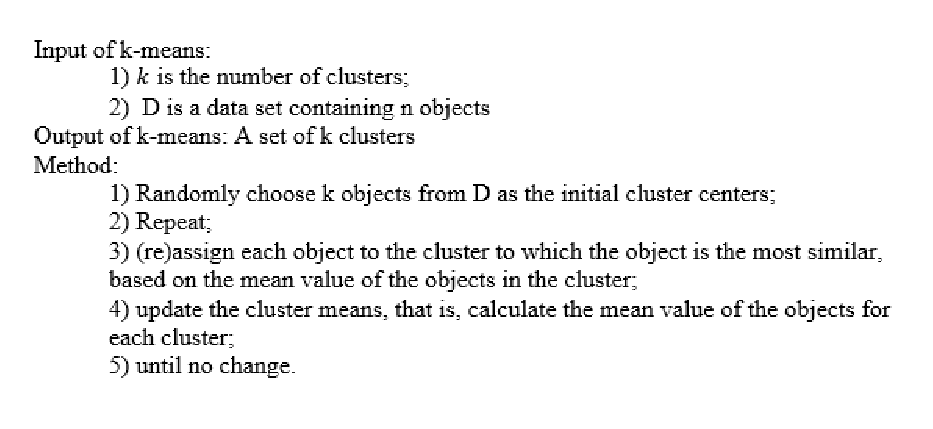
\includegraphics{alg2} 
\caption{
\label{alg2}  % use this to reference in text.
The k-means algorithm.}
\end{figure}

\subsection{Find the Right Input}
The input of the k-means algorithm, k, is very important, but the question is how the value of k is determined. In the k-means algorithm, k cluster centers are chosen at first, where k is a user-specified parameter, which is the desired number of clusters. Therefore, the number of clusters contained in the dataset is known at first. However in many cases, the distribution of the dataset is unknown. In fact, clustering is one way to find the distribution, which leads us into the contradiction of ��which came first, the chicken or the egg��. Some methods of how to effectively determine the value of k will be introduced.

The first method is to find the stabilization of a dataset. A dataset can be resampled twice to generate two subsets, and then the two subsets can be clustered by using the same algorithm, which generates two sets of k clusters. Next, the similarity of these two sets are calculated. If the degree of similarity is high, it means this k-cluster is stable and can be used for the entire dataset \cite{WFH}.

The second method is starting the k-means algorithm with k=1, and going through the process of splitting and merging. The structure will evolve its stable equilibrium state \begin{math}k_i\end{math}. It is very useful for a slightly overlapping dataset \cite{WFH}.

The next question is how to choose the appropriate initial cluster centers. One method is to choose the initial centers randomly, but this may cause poor quality of the clusters. However, the initial cluster centers can be chosen randomly multiple times, and then run each set with different random centers. Finally, the cluster with the least sum of squared errors (SSE) is chosen \cite{HanJ}.

The second effective method is to take a sample and use hierarchical clustering techniques. k clusters can be extracted from the hierarchical clustering, and used as the initial cluster centers. This method is effective, but only for the following two situations: first, the sample is relatively small; second, the value of k is relatively smaller than the size of the sample \cite{HanJ}.

Another method is to choose the first cluster center randomly or take the first points as their cluster centers. For each subsequent initial center, the point that is farthest away from the initial center is chosen. It is certain that the initial cluster center is not only random but also spread out by using this method, but beware of the outliers. In addition, the cost of finding out points farthest from the current set of initial centers is also very large. One way to overcome this problem is to use the samples, which can also reduce the amount of computation \cite{HanJ}.

Which distance measure is better becomes the next question. Euclidean distance and cosine similarity are different in mathematical logic. Euclidean distance measure is affected by different scale indicators. Therefore, generally it need to be standardized, and the greater the distance is, the greater the differences between individuals are. Cosine similarity measure in vector space is not affected by the scale indicators. The value of cosine lies in the interval [-1,1], and the larger the value is, the smaller the differences are. However, for specific applications, under what circumstances are better for using Euclidean distance or under what circumstances are better for the use of cosine similarity?

In the geometric meaning, a triangle is formed by using a segment in an n-dimensional vector space as a base and the origin as a apex, but the angle of the apex is unknown. It means that even though the distance between two vectors are certain, the value of cosine of the angle between them is still uncertain. If two vectors have the same trend, the cosine similarity tends to have better performance than Euclidean distance \cite{WFH}. For example, two vectors are (9,9) and (6,6). Obviously, these two vectors have the same trend, but the solution of Euclidean distance is way worse than cosine similarity.

If there are no points assigned to some cluster, it can form an empty cluster. A strategy is required to choose a substitute cluster center. Otherwise, the sum of squared errors will be large. One way is to choose a point farthest away from the current cluster center, which can eliminate the most impact on sum of squared errors. Another method is to choose a substitute from the cluster center with the largest sum of squared errors, which can split the clusters and reduce the sum of squared errors. If there is more than one empty cluster, the process should be repeated several times. In addition, the empty cluster may cause bugs during the programming.

\subsection{The k-means Algorithm Process}
To compute the distance on numeric data, distance measures are commonly used, which includes Minkowski distance, Euclidean distance and Manhattan distance.

The Minkowski distance between sample point \begin{math}i\end{math} and sample point \begin{math}j\end{math} is defined as
\begin{equation} d(i,j)=\sqrt[h]{\abs{x_{i1}-y_{j1}}^h+\abs{x_{i2}-y_{j2}}^h+\dots+\abs{x_{ip}-y_{jp}}^h} \end{equation}
where \begin{math} i=(x_{i1},x_{i2},\dots,x_{ip}) \end{math} and \begin{math} i=(x_{j1},x_{j2},\dots,x_{jp}) \end{math} are two \begin{math}p\end{math}-dimensional data objects, and \begin{math}h\end{math} is the order (the distance so defined is also called \begin{math}L-h\end{math} norm). Here, \begin{math}h\end{math} can be positive, negative, or even infinite. Therefore, here comes some special case of Minkowski distance when \begin{math}h\end{math} is specified. 

While \begin{math}h=1\end{math}, here comes Manhattan distance which also called as city block distance \begin{math}(L_1 norm)\end{math}. It is defined as
\begin{equation} d(i,j)=\sqrt{\abs{x_{i1}-y_{j1}}^2+\abs{x_{i2}-y_{j2}}^2+\dots+\abs{x_{ip}-y_{jp}}^2} \end{equation}
What is more, the supremum distance is generated from the Minkowsi distance for \begin{math} h\rightarrow\infty \end{math}. It is defined as
\begin{equation} d(i,j)=\lim_{h\to \infty} (\sum_{f=1}^p \abs{x_{if}-x_{jf}})^{1\over h}=\max_f \abs{x_{if}-x_{jf}} \end{equation}
There are also some important properties for these distance measures as follows:
\begin{equation} d(i,j)>0 if i \neq j, and d(i,i)=0 (Positive definiteness) \end{equation}
\begin{equation} d(i,j)=d(j,i) (Symmetry) \end{equation}
\begin{equation} d(i,j)\leq d(i,k)+d(k,j) (Triangel Inequality) \end{equation}
Last but not the least, cosine similarity can be also used for distance measure. It is defined as
\begin{equation} \cos(d_1,d_2)={(d_1 \cdot d_2) \over {\norm{d_1}\cdot\norm{d_2}}} \end{equation}
where \begin{math} d_1,d_2 \end{math} are two vectors, \begin{math} \cdot \end{math} indicates vector dot product and \begin{math} \norm{d} \end{math} is the length of vector \begin{math}d\end{math}.

The purpose of using k-means is to divide the sample into k clusters. In cluster analysis, a training set \begin{math} \{x^{(1)},x^{(2)},\dots,x^{(m)}\} \end{math} is given, where each \begin{math} x^{(i)}\in \mathbb{R}^n \end{math}. First of all, k cluster centers will be chosen randomly as \begin{math}{\mu_1,\mu_2,\dots,\mu_k} \in {\mathbb{R}^n} \end{math}.

Secondly, for every sample \begin{math}i\end{math}, each cluster that the sample belongs to should be calculated as:
\begin{equation} c^{(i)}:= arg\min_j\norm{x^{(i)}-\mu_j}^2\end{equation}
And for every cluster \begin{math}j\end{math}, the cluster centers (or mean points) of each cluster will be recalculated as:
\begin{equation} \mu_j={{\sum_{i=1}^m 1\{c^{(i)}=j\}x^{(i)}} \over {\sum_{i=1}^m 1\{c^{(i)}=j\}}} \end{equation}
Here, \begin{math}k\end{math} is the given number of clusters, and \begin{math}c^{(i)}\end{math} represents the cluster that has the shortest distance between sample \begin{math}i\end{math} and \begin{math}k\end{math} clusters, where the value of \begin{math}c^{(i)}\end{math} is ranged from 1 to k. The cluster centers (or mean points) \begin{math}\mu_j\end{math} represent the guess of the center of the samples that belongs to the same cluster.

For example, in the universe, all the stars can be divided into k constellations. To do that, first of all, k points (or k stars) in the universe are randomly chosen as cluster centers. Then the first step is to calculate each distance between each stars and k cluster centers, and choose the nearest constellations as \begin{math}c^{(i)}\end{math}. Therefore, after the first step, all the stars will have their own constellations. The next step is, for each constellations, to re-calculate their new cluster centers \begin{math}\mu_j\end{math}, which means find out the average of all the stars in each constellations. Then, repeat step one and step two until there is no change for cluster centers or the change can be ignored. Figure~\ref{fig32} shows how k-means works for n sample points, here \begin{math}k=3\end{math}.

\begin{figure}[H]
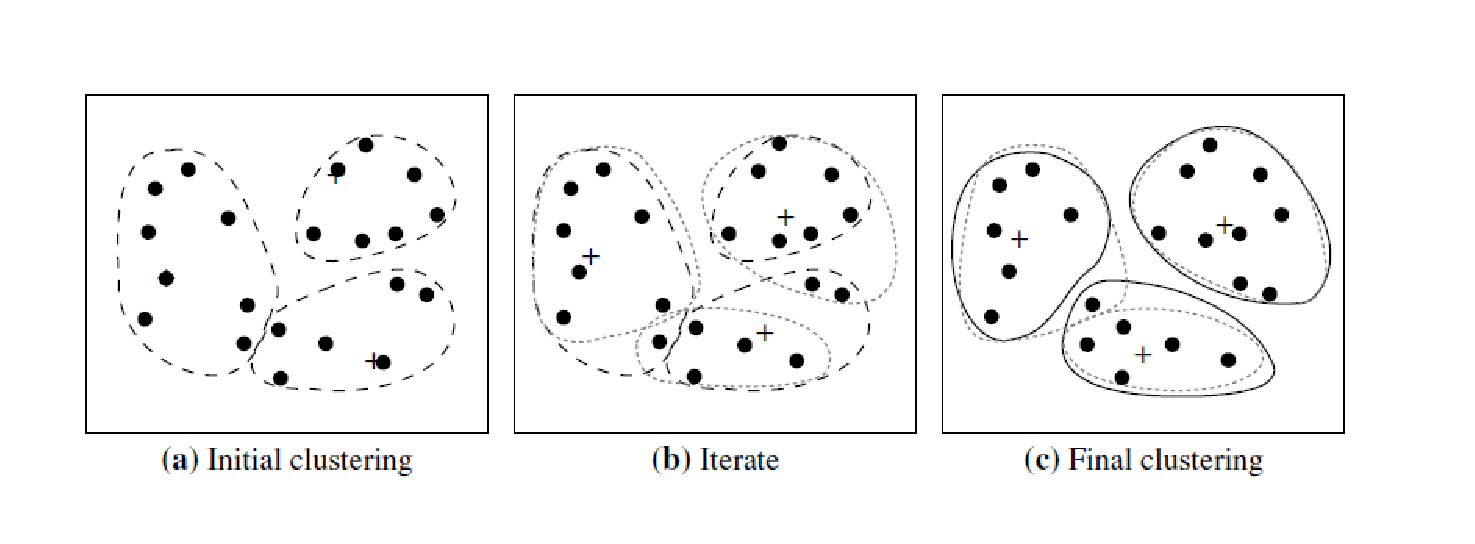
\includegraphics[width=\textwidth]{fig32} 
\caption{
\label{fig32}  % use this to reference in text.
Clustering the sample points by using the k-means algorithm.}
\centering
\end{figure}

The iteration steps of the k-means algorithm will not end until there is no change for cluster centers or the change can be ignored. In mathematical logic, it means that the algorithm will converge. As it was mentioned above, the end condition of the algorithm in the previous section is convergence. Therefore, it can prove that the k-means algorithm can ensure the convergence. Next, for figuring out the convergence, distortion function will be defined as follows:
\begin{equation} J(c,\mu)=\sum_{i=1}^m \norm{x{(i)}-\mu_{c^{(i)}}}^2 \end{equation}
The function \begin{math}J\end{math} means the sum of squares of the distances between each sample points and their cluster centers, so the purpose of the k-means algorithm is to minimize the function \begin{math}J\end{math}. Assume that before the function \begin{math}J\end{math} reaches its minimum, the cluster center \begin{math} \mu_j \end{math} of each cluster can not be changed and the cluster \begin{math} c^{(i)} \end{math} that the sample points belong to can adjusted for the reduction of the function \begin{math}J\end{math}. In the same manner, the cluster \begin{math} c^{(i)} \end{math} that the sample points belong to can be fixed and the cluster center \begin{math} \mu_j \end{math} of each cluster can be adjusted for the reduction of the function \begin{math}J\end{math}. These two processes can make sure that the function \begin{math}J\end{math} will monotonically decrease within the loop. When the function \begin{math}J\end{math} achieve to its minimum, \begin{math} \mu \end{math} and \begin{math}c\end{math} also converge. Theoretically, there are many different pairs of \begin{math} \mu \end{math} and \begin{math}c\end{math} that make the function J reach its minimum, but they are rare practically.

Since the distortion function \begin{math}J\end{math} is a non-convex function, it means that it is not guaranteed that the obtained minimum value is the global minimum. Therefore, it is really picky and tricky how the initial cluster centers of the k-means algorithm are chosen, but generally the local minimum, achieved by the k-means algorithm, is enough to meet the requirement. If the local minimum does not meet the requirement, the different initial value of the k-means algorithm can be chosen and find out the corresponding \begin{math} \mu \end{math} and \begin{math}c\end{math} of the minimum \begin{math}J\end{math} among the different cases.

\section{Support Vector Machine (SVM)}
\subsection{Introduction}
Data classification is one of the most important subjects in data mining. Data classification is based on some existing training data, and then generates a trained classifier according to some theory. Next, the trained classifier is used to test the unknown data to find out a new classification.

One of these theories is Support Vector Machine (SVM). SVM is first proposed by Cortes and Vapnik in 1995. SVM has its advantage of solving the problem of nonlinear and high dimensional pattern recognition, and be able to extend the use to other machine learning problems, such as the function fitting \cite{HanJ}. SVM is a method for the classification of both linear and nonlinear data. It uses a nonlinear mapping to transform the original training data into a higher dimension. Within this new dimension, it searches for the linear optimal separating hyperplane. With an appropriate nonlinear mapping to a sufficiently high dimension, data from two classes can always be separated by a hyperplane. The SVM finds this hyperplane using support vectors and margins. The data mining algorithm SVM is capable of finding the maximum margin for image pattern recognition with high classification accuracy and limited architecture design \cite{MGLM}. 


Support Vector Machine is also a method that is based on the boundary classification. The basic principle of SVM can be defined as follows. For the better understanding, two-dimensional data is taken as an example. If all the points of a training data is distributed on a two-dimensional plane, they are gathered in different areas according to its own classification. The goal of those classification algorithm based on the boundary classification is to find the boundary between the classifications through training. If the boundary is a straight line, this case is linear; if the boundary is a curve, this case is considered as non-linear. For the multi-dimensional data, such as N-dimensional, they can be regarded as the points in the N-dimensional space, and the boundary in such space is (N-1)-dimensional plane. Thus, linear classifier in multi-dimensional data is a hyper-plane, and non-linear classifier in multi-dimensional data is a hyper-curve.

Linear classifier is shown in the following Figure~\ref{fig21}. According to the position of the new data point against the boundary, its classification can be determined. Here is the example of only two classifications, but it can be easily extended to multi-classification.

\begin{figure}[H]
\centering
\includegraphics[width=\textwidth]{fig21} 
\caption{
\label{fig21}  % use this to reference in text.
Linearly separable data.}
\end{figure}

\subsection{The SVM Process}
All the support vector machine are based on a linear classifier, but not all the data can be linearly separated. For example, in a two-dimensional plane, all the points that belongs to two classifications can be separated by a curve. Therefore, all the points in a low-dimensional space can be mapped into high-dimensional space by using SVM, and in the high-dimensional space, all the points are now linearly separated. The boundary of two classification can be determined by a linear classifier now. In a high-dimensional space, it is a linear classifier; in the original dimensional space, it is a non-linear classifier.

The algorithm of mapping from a low-dimensional space to a high-dimensional space is not the key to SVM, and these algorithms are given the kernel functions, which includes Polynomial kernel of degree \begin{math}h\end{math}, Gaussian radial basis function kernel and Sigmold kernel. SVM is considered as an optimization problem, which means to find out the optimal solution.

Assume that the problem is considered as a function \begin{math} f(x) \end{math}. To find out the optimal solution is to find out the minimum value of the function \begin{math} f(x) \end{math}. Since \begin{math} f(x) \end{math} is not always continuously differentiable, the solution can not be found by finding the points where derivative equals to zero. The optimization problems can be divided into two categories: unconstrained optimization and constrained optimization. Unconstrained optimization can be expressed as 
\begin{equation} \min_x f(x) \end{equation},
and constrained optimization can be expressed as
\begin{equation}
\left\{\begin{matrix}
min_x f(x) & x \in E^n\\ 
s.t.\text{ } \varphi_i(x)\geq0 & i \in \{1,2,\dots,m\}
\end{matrix}\right.\end{equation}

\subsection{Linearly Separable}
From Figure~\ref{fig21}, the white points are class 1, the black points are class 2, and there are several straight lines that separate these two classifications are represented as \begin{math}f(x)=k\cdot x+b\end{math}, where both k and b are vectors. Therefore, they can also be written in the form of \begin{math}f(x)=k_1\cdot x_1+ k_2\cdot x_2+\dots+k_n\cdot x_n+b\end{math}. When the dimension of vector x is 2, \begin{math}f(x)\end{math} is a straight line in a two-dimensional plane; when the dimension of vector x is 3, \begin{math}f(x)\end{math} is a plane in a two-dimensional space; when the dimension of vector x is greater than 3, \begin{math}f(x)\end{math} is an (n-1)-dimensional hyper-plane in an n-dimensional space. Here, sign function will used to determine which classification the points belong to. When \begin{math}f(x)\end{math} is greater than zero, \begin{math}sign(f(x))\end{math} is +1; when \begin{math}f(x)\end{math} is less than zero, \begin{math}sign(f(x))\end{math} is -1. As shown in the Figure~\ref{fig21}, the y value of the white points is +1, and the y value of the black points is -1.

However, there are several lines that can separate these two classifications, so how to determine the optimal one is the key to SVM. In Figure~\ref{fig22}, there are two possible separating hyper-planes and their margins.

\begin{figure}[H]
\centering
\includegraphics[width=\textwidth]{fig22} 
\caption{
\label{fig22}  % use this to reference in text.
Two possible linearly separable cases.}
\end{figure}

Intuitively speaking, the larger the margin is, the better the case is. So, maximum marginal hyper-plane is one of the most important conditions in the SVM theory. It makes more sense that the linear classifier with the largest margin is chosen. From a probabilistic point of view, it makes the points with the least confidence have the most confidence. The points on the dash lines are called support vectors, and the straight line in the middle is called classifier boundary \begin{math}sign(f(x))\end{math}. If M is the margin width, M can be defined as \begin{equation} M={2 \over \sqrt{k \cdot k}} \end{equation}
Therefore, the problem is transferred into finding out the optimization:
\begin{equation} \max{1 \over \norm{k}} \rightarrow \min{{1 \over 2} \norm{k}^2} \end{equation}
where \begin{math}\norm{k}\end{math} is the Euclidean norm of k, which also equal to \begin{math}\sqrt{ k \cdot k }\end{math}. Therefore, the original SVM problem is also the optimization problem:
\begin{equation}
\left\{\begin{matrix}
\min{{1 \over 2} \norm{k}^2}\\ 
s.t.\text{   }y_i(k^Tx_i+b)\geq 1,\text{ }i=1,2,\dots,n
\end{matrix}\right.
\end{equation}

\subsection{Linearly Inseparable}
Since there are too many limitations of linearly separable cases in reality, linearly inseparable cases are mentioned here in Figure~\ref{fig23}.

\begin{figure}[H]
\centering
\includegraphics[width=\textwidth]{fig23} 
\caption{
\label{fig23}  % use this to reference in text.
Linearly inseparable data.}
\end{figure}

In order to do the classification in this case, there are two ways: one is to use the straight line or hyper-plane, but it is not guaranteed that all the points should be separated according to the classification. However, the error is not guaranteed also; the other is to use the curve to completely separate all the points, and it is associated with the kernel function.

Since the error of the first method is not guaranteed, here the second method is detailed. In the Figure~\ref{fig23}, it is not possible to separate all the points by using a straight line, so the original input data has to be transferred into a higher dimensional space for linearly separation. However, the nonlinear mapping to a higher dimensional space is uncertain, and the computation involved may be costly. There are three admissible kernel functions (shown in Figure~\ref{fig24}) with which can be replaced anywhere \begin{math} \phi(X_i)  \cdot \phi(X_j) \end{math}shows in the algorithm.

\begin{figure}[H]
\centering
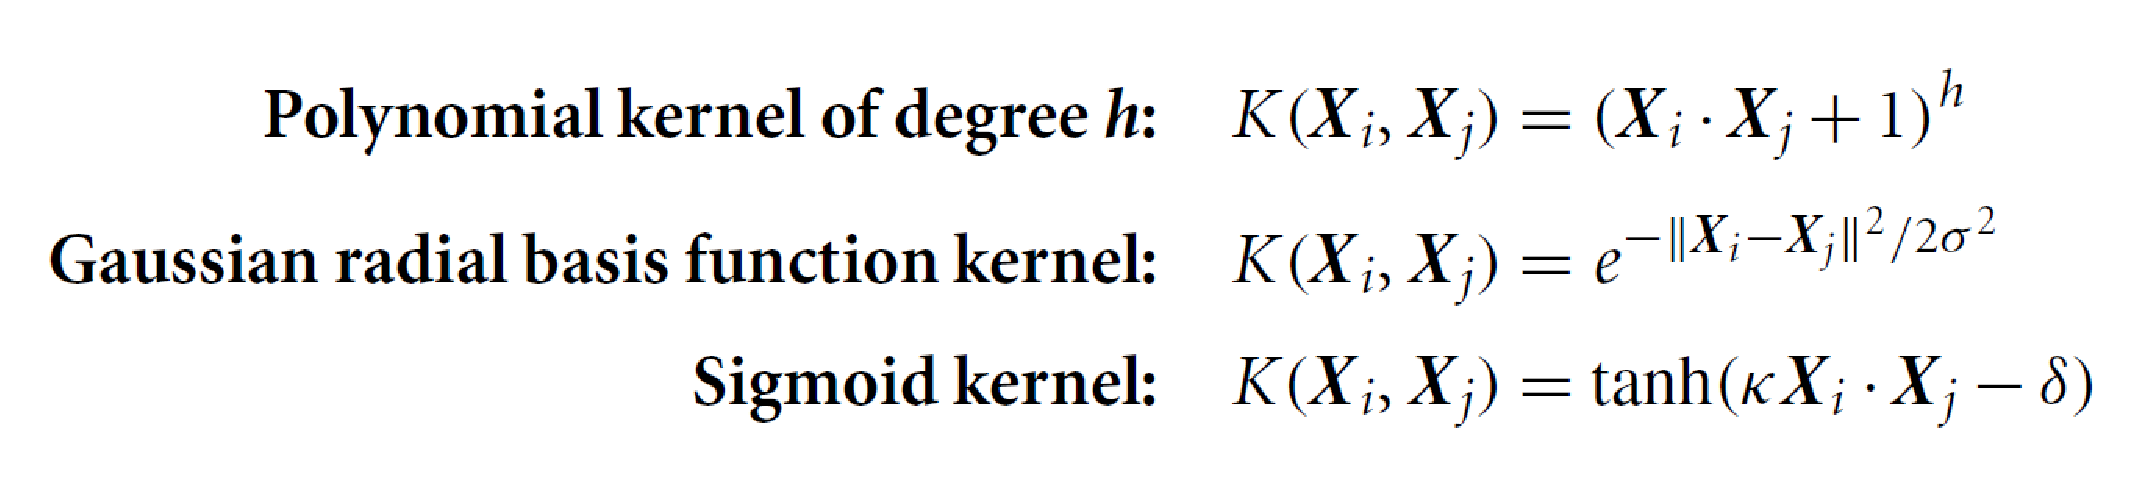
\includegraphics[width=\textwidth]{fig24} 
\caption{
\label{fig24}  % use this to reference in text.
Three kernel functions.}
\end{figure}

\subsection{Multiple classification (N-classification)}
In the case of multiple classification, there are two basic methods: one is 1 vs (N-1) method; the other is 1 vs 1 method.

In the first method, N classifiers are trained, and whether \begin{math}i\end{math}-th classifier belongs to classification \begin{math}i\end{math} or other classifications is checked. To identify an \begin{math}x\end{math}, a classification with the largest \begin{math}g^j(x)\end{math} is where \begin{math}i\end{math} belongs to. \begin{math} g^j(x)\end{math} is defined as
\begin{equation} g^j(x)=\sum_{i=1}^{j}a_i^jy_iK(x,x_i)+b^j \end{equation}

In the second method, \begin{math}N*(N-1)/2 \end{math} classifiers are trained. To identify an \begin{math}x \end{math}, a vote method is used. The classification with the most votes finally gets \begin{math}x\end{math}.


%chapter4
\chapter{Experimental Results}
The hyperspectral image of the mud sample mentioned in Chapter 1 is used as the input data (raw data) of the hybrid system. The dataset is an 811-band 50-by-1600 hyperspectral image of a mud sample, whose pixel values are band interleaved by line (BIL) in order of increasing band number. BIL is one of three primary methods for encoding multiband image data, which has the advantage of accessing the spatial and spectral data easily.

\section{Apply Vegetation Detection Algorithm}
To find out the three most informative bands is the first step. The MATLAB function multibandread is one of the most important functions to read in the hyperspectral image. Therefore, an RGB image is imported into MATLAB, which red means the NIR band, green means the visible red band and blue means the visible green band. Figure~\ref{fig41} and ~\ref{fig42} show the color infrared image.

\begin{figure}[H]
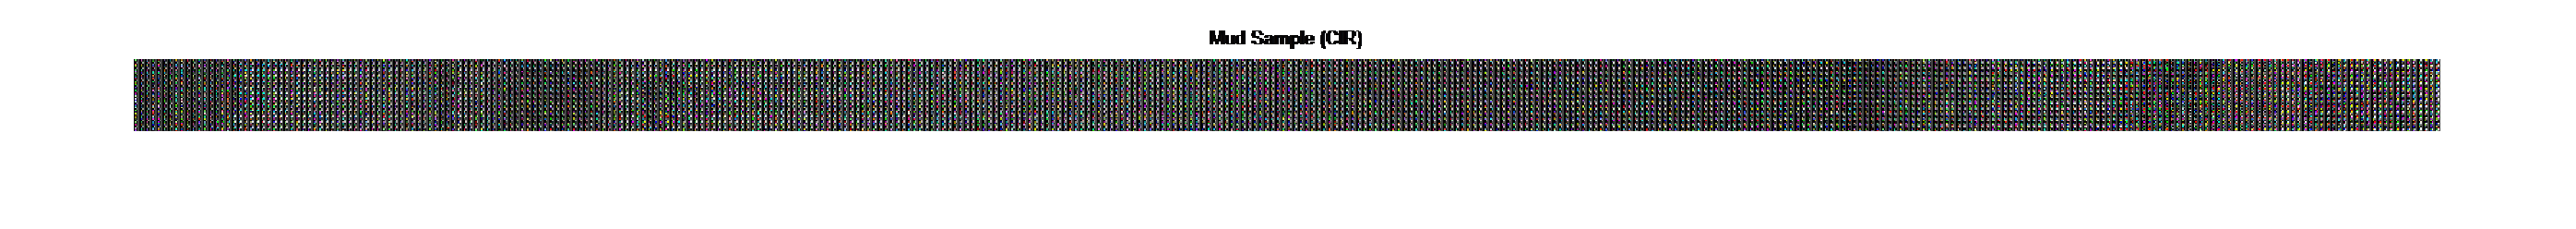
\includegraphics[width=\textwidth]{fig41} 
\caption{
\label{fig41}  % use this to reference in text.
Entire color infrared (CIR).}
\centering
\end{figure}

\begin{figure}[H]
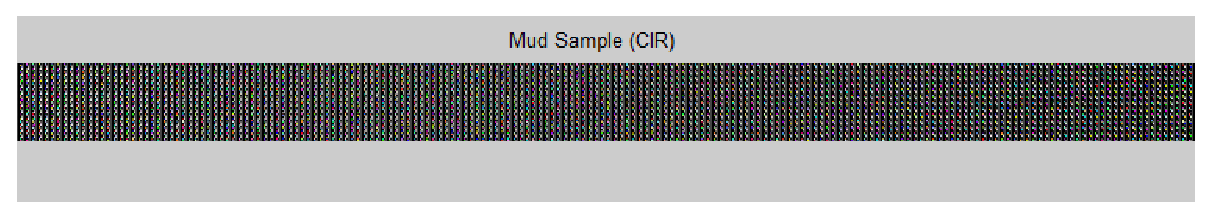
\includegraphics[width=\textwidth]{fig42} 
\caption{
\label{fig42}  % use this to reference in text.
Zoom in of CIR.}
\centering
\end{figure}

Decorrelation stretch is applied in the previous CIR image for better display. Decorrelation stretch can highlight the elements in a multichannel image by exaggerating the color differences. It is pretty wise to use option \lq Tol\rq in decorrelation stretch, which can linearly contrast stretch. Tol = [LOW\_FRACT HIGH\_FRACT] specifies the fraction of the image to saturate at low and high intensities. Therefore, Tol is specified as 0.01, saturating at low and high intensities by one percent. Figure~\ref{fig43} and ~\ref{fig44} show the color infrared image with decorrelation stretch.

\begin{figure}[H]
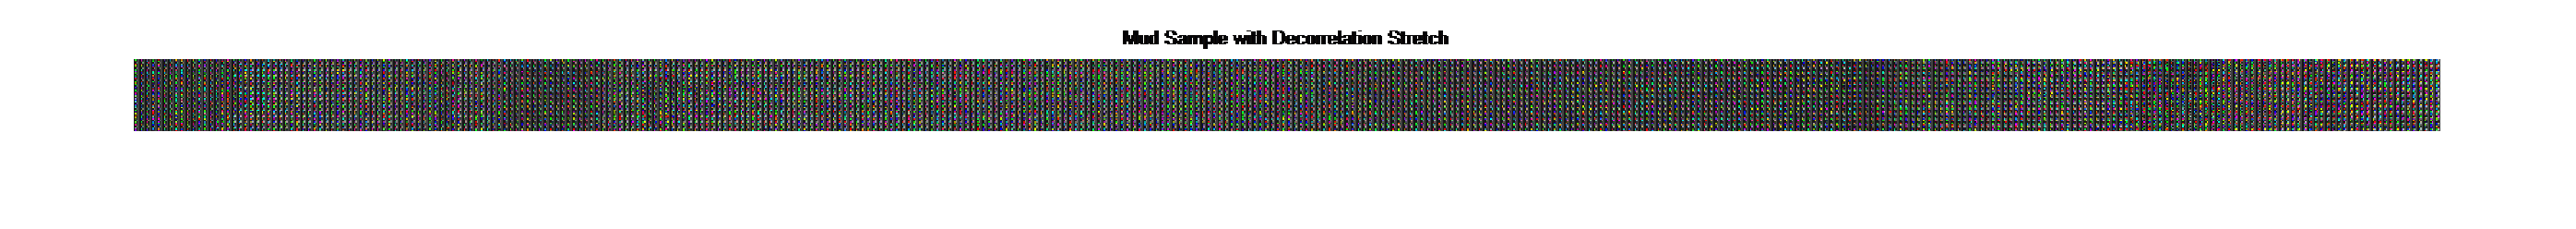
\includegraphics[width=\textwidth]{fig43} 
\caption{
\label{fig43}  % use this to reference in text.
Entire color infrared (CIR) with decorrelation stretch.}
\centering
\end{figure}

\begin{figure}[H]
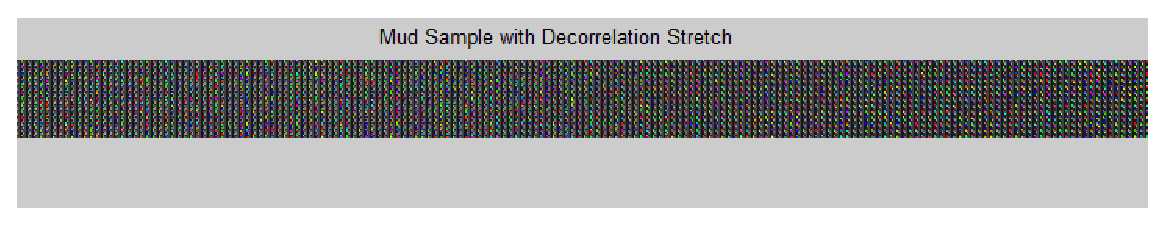
\includegraphics[width=\textwidth]{fig44} 
\caption{
\label{fig44}  % use this to reference in text.
Zoom in of CIR with decorrelation stretch.}
\centering
\end{figure}

An NIR-Red scatter plot is constructed to help us compare the NIR band (displayed as red) and the visible red band (displayed as green). As we said above, we can easily extract the NIR and red bands from the CIR composite. So we can see the difference between these two bands in grayscale images. Figure~\ref{fig45}, ~\ref{fig46}, ~\ref{fig47} and ~\ref{fig48} show the near infrared band image and the visible red band image.

\begin{figure}[H]
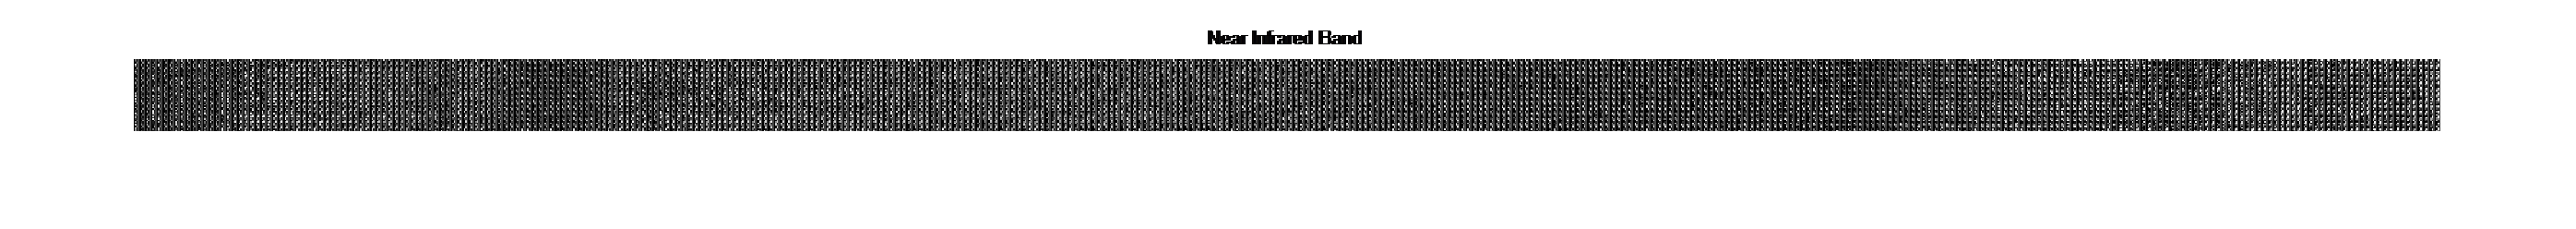
\includegraphics[width=\textwidth]{fig45} 
\caption{
\label{fig45}  % use this to reference in text.
Entire near infrared (NIR) band.}
\centering
\end{figure}

\begin{figure}[H]
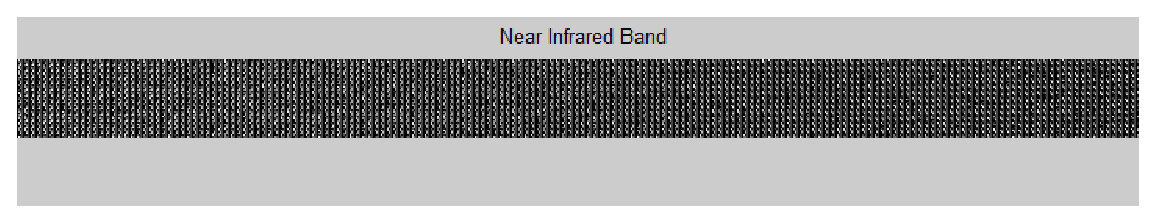
\includegraphics[width=\textwidth]{fig46} 
\caption{
\label{fig46}  % use this to reference in text.
Zoom in of NIR band.}
\centering
\end{figure}

\begin{figure}[H]
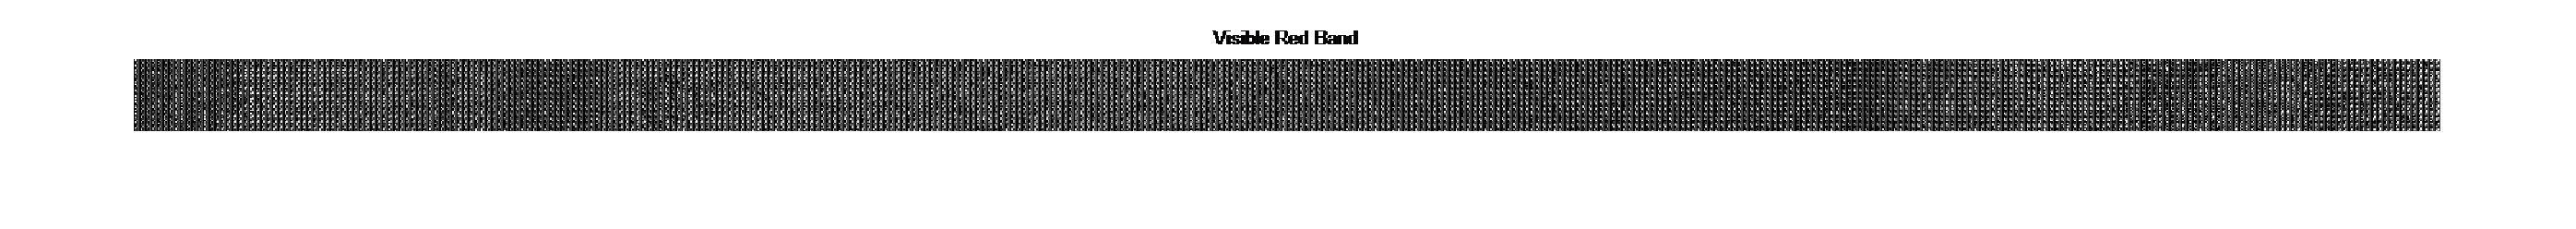
\includegraphics[width=\textwidth]{fig47} 
\caption{
\label{fig47}  % use this to reference in text.
Entire visible red band.}
\centering
\end{figure}

\begin{figure}[H]
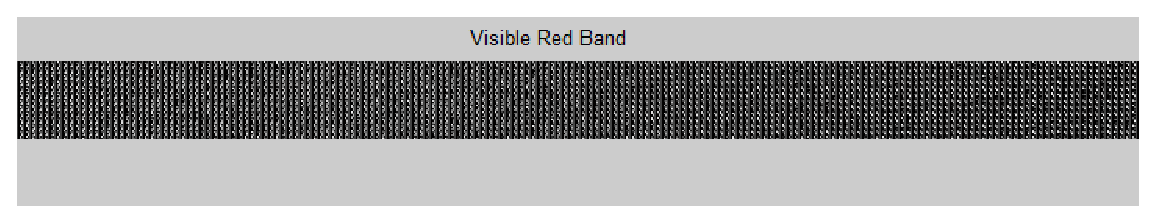
\includegraphics[width=\textwidth]{fig48} 
\caption{
\label{fig48}  % use this to reference in text.
Zoom in of visible red band.}
\centering
\end{figure}

Using the MATLAB function plot, we can easily have the scatter plot of each pixel with red level vs NIR level. For the purpose of the further computation, we scale the red level and NIR level values from 0 to 1. Figure~\ref{fig49} shows the scatter plot of visible red band and NIR band.

\begin{figure}[H]
\centering
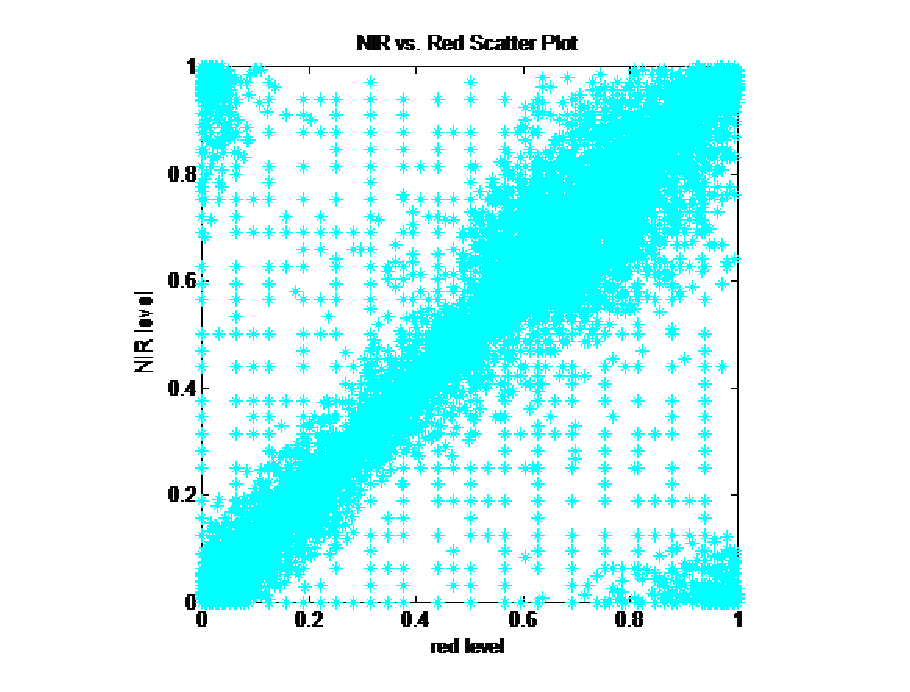
\includegraphics{fig49} 
\caption{
\label{fig49}  % use this to reference in text.
NIR band vs visible red band.}
\end{figure}

From the scatter plot, most of pixels are along the diagonal, which means the NIR and red values are nearly the same. Also, we have some pixels at corners, which are the significant objects or pixels we are looking for.

To find out the significant objects, we have to compute the index of each pixel:
\begin{equation} \text{Index = {(NIR - red) ./ (NIR + red)}} \end{equation}

From this equation, if index approaches to 0, pixels are along the diagonal; if index approaches to 1, pixels are at top left corner; if index approaches to -1, pixels are at bottom right corner. Figure~\ref{fig410} and ~\ref{fig411} show the normalized difference image by using the index equation.

\begin{figure}[H]
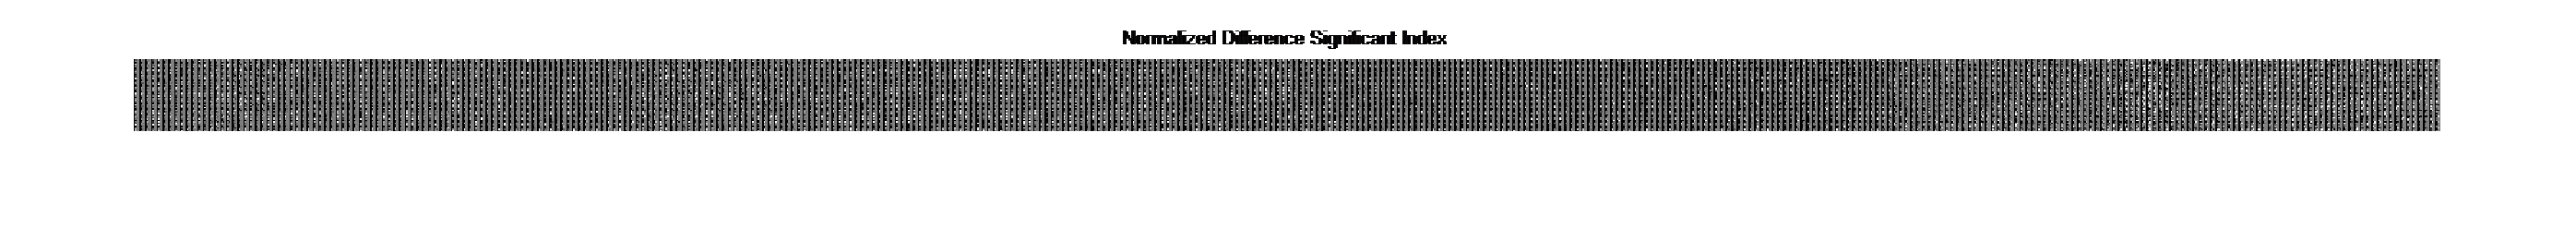
\includegraphics[width=\textwidth]{fig410} 
\caption{
\label{fig410}  % use this to reference in text.
Normalized difference image by using the index equation.}
\centering
\end{figure}

\begin{figure}[H]
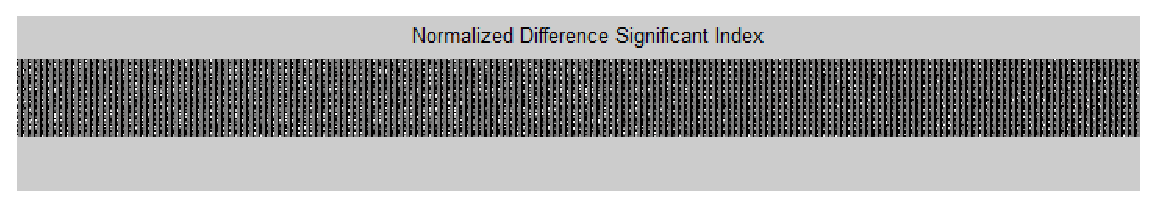
\includegraphics[width=\textwidth]{fig411} 
\caption{
\label{fig411}  % use this to reference in text.
Zoom in of normalized difference image by using the index equation.}
\centering
\end{figure}

In order to identify pixels most likely to contain significant objects, we apply a simple threshold to the previous image. We just need to create the significant objects image that have index greater than threshold. Figure~\ref{fig412} and ~\ref{fig413} show the index image with threshold applied.

\begin{figure}[H]
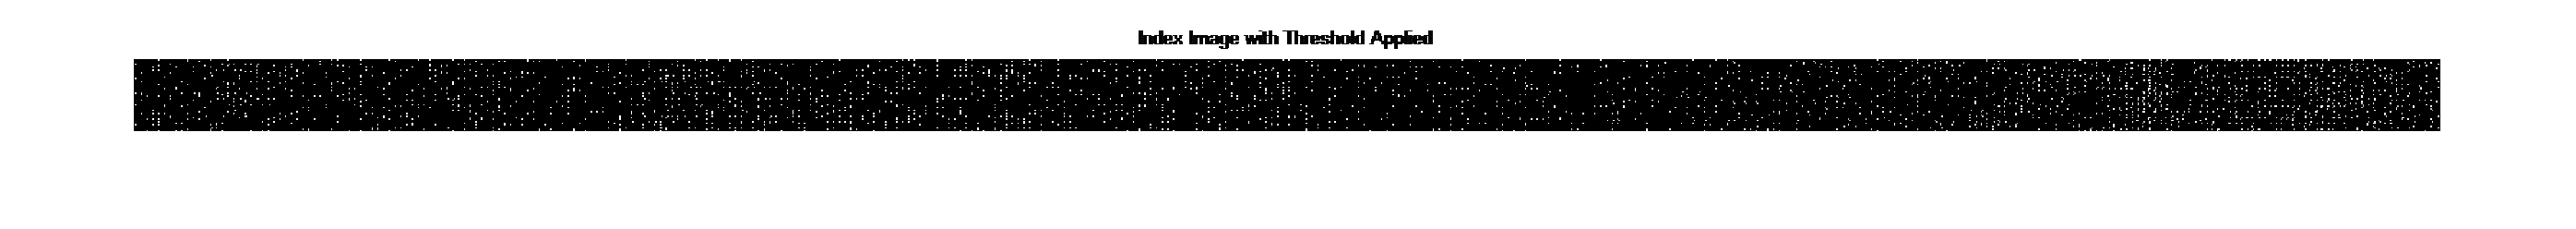
\includegraphics[width=\textwidth]{fig412} 
\caption{
\label{fig412}  % use this to reference in text.
Index image with threshold applied.}
\centering
\end{figure}

\begin{figure}[H]

\includegraphics[width=\textwidth]{fig413} 
\caption{
\label{fig413}  % use this to reference in text.
Zoom in of index image with threshold applied.}
\centering
\end{figure}

Finally, we re-draw the useful scatter plot and the index image with threshold applied for better display. Figure~\ref{fig414} and ~\ref{fig415} show the colored scatter plot and index image with threshold applied.

\begin{figure}[H]
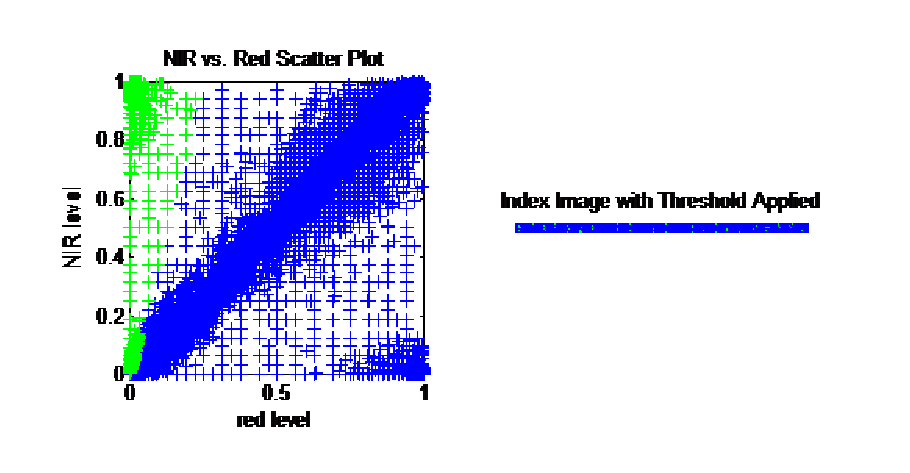
\includegraphics[width=\textwidth]{fig414} 
\caption{
\label{fig414}  % use this to reference in text.
Scatter Plot of NIR vs Red band and Index image with threshold applied with color. The green part is the significant objects; the blue part is the mud.}
\centering
\end{figure}

\begin{figure}[H]

\includegraphics[width=\textwidth]{fig415} 
\caption{
\label{fig415}  % use this to reference in text.
Zoom in of Index image with threshold applied with color.}
\centering
\end{figure}

Percentage of significant objects is calculated by ratio of number of while pixels in binary image to total number of pixels in NIR image. It was found to be 3.5438\%.

\section{Apply the k-means Algorithm}
The dataset here is the same as the one before. However, the hyperspectral image is read in single precision, and mathematically, the dataset is stored in two dimensional by having each column display the entire pixel values of each layer or band. Since the second method of how to determine k and the percentage of significant objects is used, here is the result of the k-means algorithm as follows: (start from \begin{math}k=2\end{math})

If \begin{math}k=2\end{math}, it means that the result only has two clusters. The measured time for running the model is 200.49600 seconds. The hyperspectral image is divided into two clusters, one includes 34640 (43\%) and the other includes 45360 (57\%). If we see the original photo, we can see the tapes along the sides of the picture. It is reasonable that the 43\% is the tape and that the 57\% is the mud sample. Since the sum of squared errors of \begin{math}k=2\end{math} is 731482.1304914309, the mud sample definitely can be divided into more clusters. Figure~\ref{fig416} shows the k-means algorithm with \begin{math}k=2\end{math}.

\begin{figure}[H]
\centering
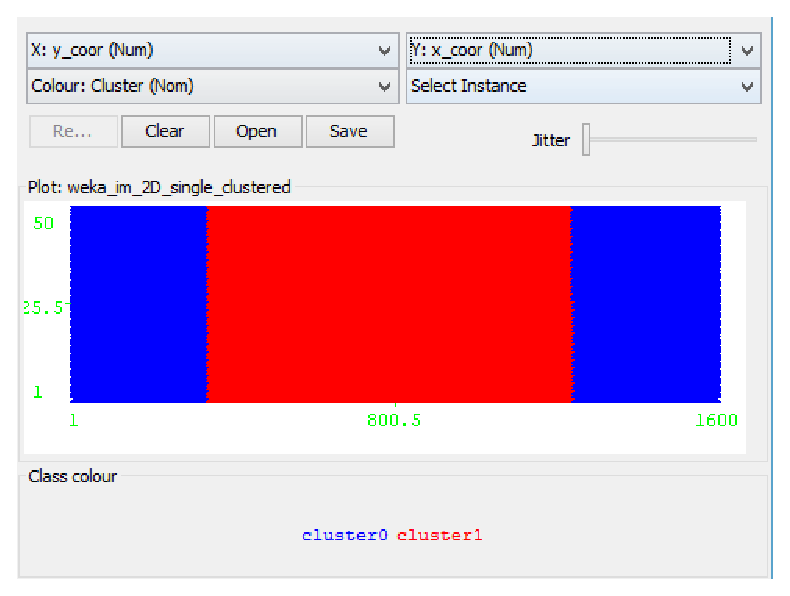
\includegraphics{fig416} 
\caption{
\label{fig416}  % use this to reference in text.
The k-means algorithm with k=2.}
\end{figure}

If \begin{math}k=3\end{math}, it means that the result only has three clusters. The measured time for running the model is 703.78100 seconds, and it is significantly increased from \begin{math}k=2\end{math}. The hyperspectral image is divided into three clusters, 33441 (42\%), 11029 (14\%) and 35530 (44\%). It is still reasonable that the 42\% is the tape and that the rest 58\% is the mud sample with one more cluster. Figure~\ref{fig417} shows the k-means algorithm with \begin{math}k=3\end{math}.

\begin{figure}[H]
\centering
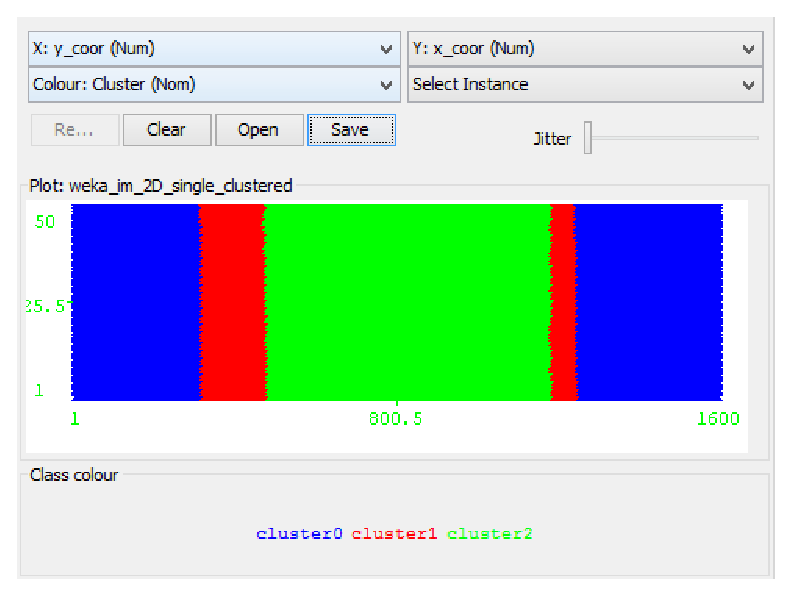
\includegraphics{fig417} 
\caption{
\label{fig417}  % use this to reference in text.
The k-means algorithm with k=3.}
\end{figure}

If \begin{math}k=4\end{math}, it means that the result only has four clusters. The measured time for running the model is 858.32800 seconds. The hyperspectral image is divided into four clusters, 33132 (41\%), 11105 (14\%), 31009 (39\%) and 4754 (6\%). It is still reasonable that the 41\% is the tape and that the rest 59\% is the mud sample with two more clusters. It is noticed that the 6\% cluster may be have some association with the significant objects and that the sum of squared errors of \begin{math}k=4\end{math} is 138644.72818111547. Although the sum of squared errors is significantly reduced compared to \begin{math}k=2\end{math}, it is not stable yet. Figure~\ref{fig418} shows the k-means algorithm with \begin{math}k=4\end{math}.

\begin{figure}[H]
\centering
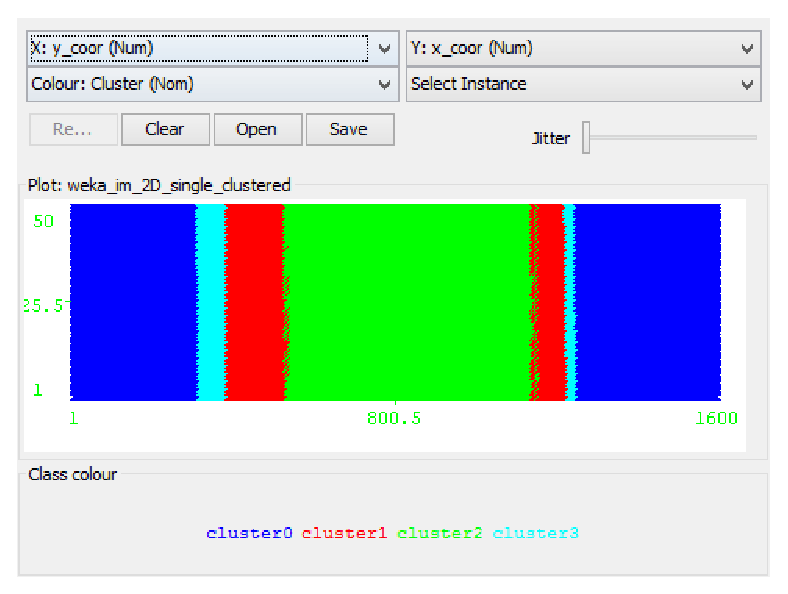
\includegraphics{fig418} 
\caption{
\label{fig418}  % use this to reference in text.
The k-means algorithm with k=4.}
\end{figure}

The measured time for running the model of \begin{math}k=8\end{math} is 1442.11500 seconds. The hyperspectral image is divided into eight clusters, 12882 (16\%), 4537 (6\%), 6740 (8\%), 5238 (7\%), 9517 (12\%), 23895 (30\%), 2237 (3\%) and 14954(19\%). It is noticed that the 3\% cluster is below the percentage of the significant objects we got from the last section and that may be have some association with the significant objects. But the sum of squared errors of \begin{math}k=8\end{math} is 61049.33552500921, and it is not stable yet. Figure~\ref{fig419} shows the k-means algorithm with \begin{math}k=8\end{math}.

\begin{figure}[H]
\centering
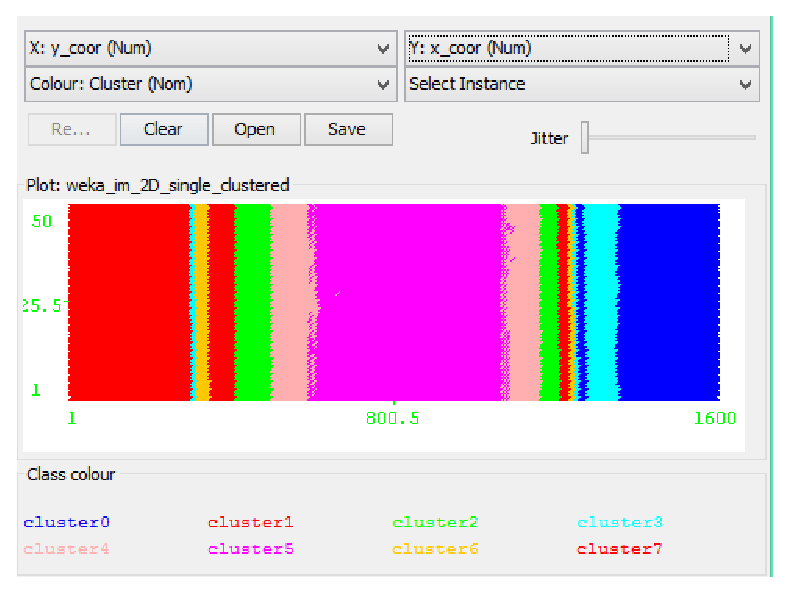
\includegraphics{fig419} 
\caption{
\label{fig419}  % use this to reference in text.
The k-means algorithm with k=8.}
\end{figure}

The measured time for running the model of \begin{math}k=12\end{math} is 1456.19100 seconds. The hyperspectral image is divided into twelve clusters, 6491 (8\%), 5978 (7\%), 6910 (9\%), 5114 (6\%), 10693 (13\%), 15891 (20\%), 1202 (2\%), 7449 (9\%), 2445 (3\%), 3861(5\%), 7509 (9\%) and 6457 (8\%). It is noticed that some clusters are below the percentage of the significant objects we got from the last section and that may be have some association with the significant objects. But the sum of squared errors of \begin{math}k=12\end{math} is 40940.46539080349, and still it is not stable yet. Figure~\ref{fig420} shows the k-means algorithm with \begin{math}k=12\end{math}.

\begin{figure}[H]
\centering
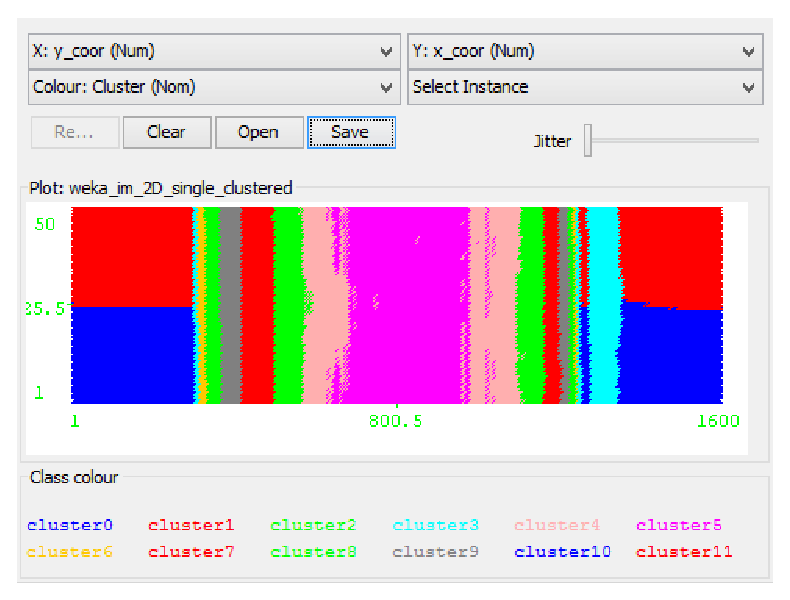
\includegraphics{fig420} 
\caption{
\label{fig420}  % use this to reference in text.
The k-means algorithm with k=12.}
\end{figure}

The measured time for running the model of \begin{math}k=16\end{math} is 1713.76900 seconds. The hyperspectral image is divided into sixteen clusters, 6370 (8\%), 3707 (5\%), 4405 (6\%), 712 (1\%), 9822 (12\%), 14089 (18\%), 1339 (2\%), 2784 (3\%), 1954 (2\%), 2856(4\%), 5352 (6\%), 5169 (6\%), 6457 (8\%), 5055 (6\%), 6855 (9\%) and 3074 (4\%). It is noticed that some clusters are below the percentage of the significant objects we got from the last section and that may be have some association with the significant objects. The sum of Squared Error of 16 clusters: 30656.364971050734, and still it is stable. Figure~\ref{fig421} shows the k-means algorithm with \begin{math}k=16\end{math}.

\begin{figure}[H]
\centering
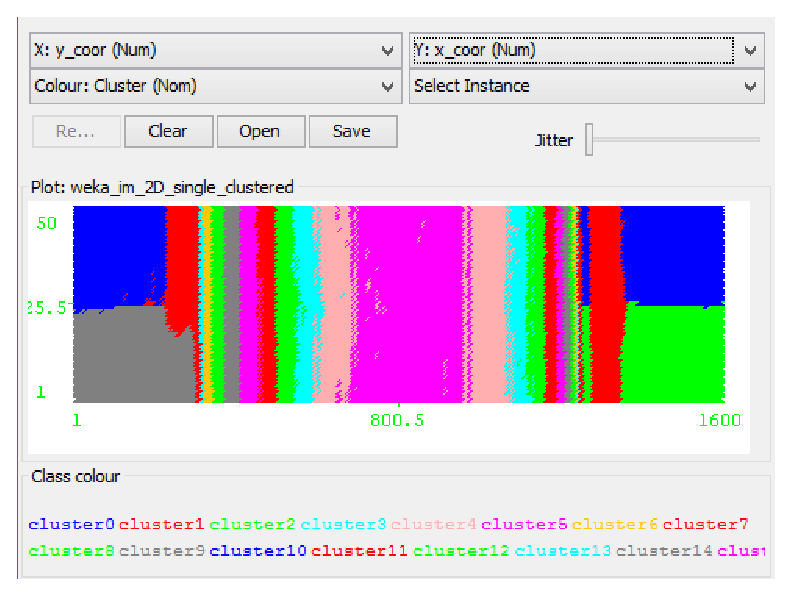
\includegraphics{fig421} 
\caption{
\label{fig421}  % use this to reference in text.
The k-means algorithm with k=16.}
\end{figure}

Table~\ref{tab1} shows results of the k-means algorithm from \begin{math}k=2\end{math} to \begin{math}k=24\end{math}, which includes the sum of squared error, percentage of clusters and running time. 

\makeatletter
\def\hlinewd#1{%
\noalign{\ifnum0=`}\fi\hrule \@height #1 %
\futurelet\reserved@a\@xhline}
\makeatother

\begin{center}
\begin{longtable}[H]{| C{1.9cm} | C{3.8cm} | C{5cm} | C{2.8cm} |}
\hline 
Number of Clusters & Sum of Squared Error & Percentage of Clusters & Running Time (seconds)\\ [0.5ex] 
%heading
\hlinewd{2pt}
2 & 731482.1304914309 & 34640(43\%) and 45360(56\%) & 200.49600 \\ [1ex]
\hline
3 & 250413.2621864793 & 33441(42\%), 11029(14\%) and 35530(44\%) & 703.78100 \\ [1ex]
\hline
4 & 138644.72818111547 & 33132(41\%), 11105(14\%), 31009(39\%) and 4754(6\%) & 858.32800 \\ [1ex]
\hline
8 & 61049.33552500921 & 12882(16\%), 4537(6\%), 6740(8\%), 5238(7\%), 9517(12\%), 23895(30\%), 2237(3\%) and 14954(19\%) & 1442.11500 \\ [1ex]
\hline
12 & 40940.46539080349 & 6491(8\%), 5978(7\%), 6910(9\%), 5114(6\%), 10693(13\%), 15891(20\%), 1202(2\%), 7449(9\%), 2445(3\%), 3861(5\%), 7509(9\%) and 6457(8\%) & 1456.19100 \\ [1ex]
\hline
16 & 30656.364971050734 & 6370(8\%), 3707(5\%), 4405(6\%), 712(1\%), 9822(12\%), 14089(18\%), 1339(2\%), 2784(3\%), 1954(2\%), 2856(4\%), 5352(6\%), 5169(6\%), 6457(8\%), 5055(6\%), 6855(9\%) and 3074(4\%) & 1713.76900 \\ [1ex]
\hline
20 & 28912.487844715703 & 6174(7\%), 2866(3\%), 3309(4\%), 756(0\%), 7296(9\%), 7369(9\%), 1143(1\%), 2650(3\%), 1506(1\%), 1754(2\%), 4911(6\%), 5434(6\%), 6247(7\%), 4950(6\%), 2551(3\%), 2214(2\%), 279(0\%), 4885(6\%), 9362(11\%) and 4344(5\%) & 6030.18200 \\ [1ex]
\hline
24 & 26249.48621819265 & 5229(6\%), 3600(4\%), 2890(3\%), 2503(3\%), 4639(5\%), 6802(8\%), 1224(1\%), 2255(2\%), 1825(2\%), 2822(3\%), 3472(4\%), 2460(3\%), 5154(6\%), 4122(5\%), 3232(4\%), 3006(3\%), 2595(3\%), 3639(4\%), 4640(5\%), 3924(4\%), 786(0\%), 6547(8\%), 278(0\%) and 2356(2\%) & 6376.13100 \\ [1ex]
\hline
\caption{The results of the k-means algorithm from k=2 to k=24} 
\label{tab1}
\end{longtable}
\end{center}

Since the sum of squared errors from \begin{math}k=2\end{math} to \begin{math}k=24\end{math} are available, a curve fitting can be applied for them. Figure~\ref{kmeans_error} shows curve fitting of the number of clusters versus the sum of squared error. According to the curve fitting, \begin{math}k=16\end{math} has the stable sum of squared error.

\begin{figure}[H]
\centering
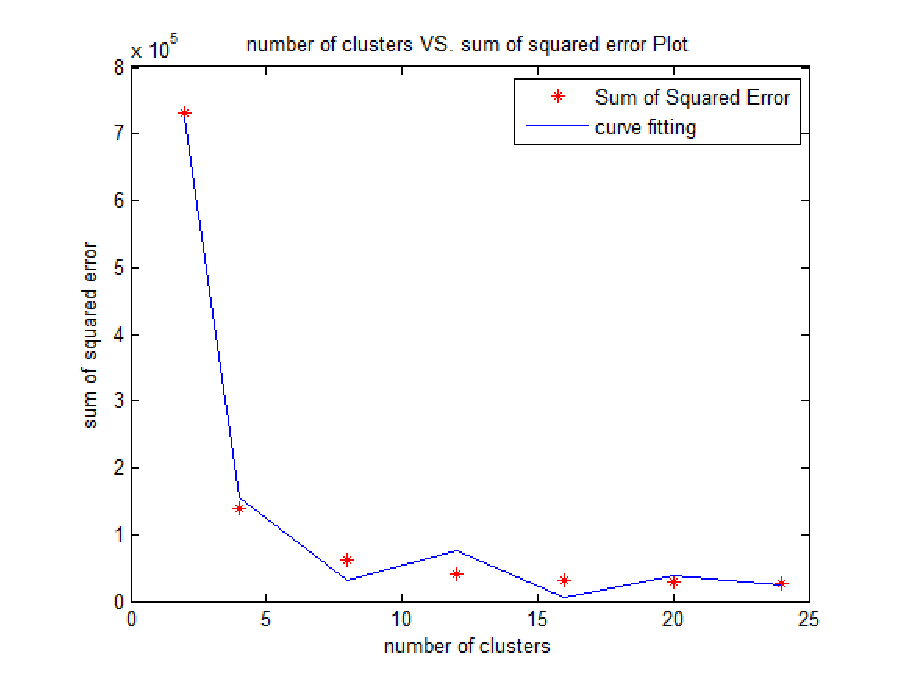
\includegraphics{kmeans_error} 
\caption{
\label{kmeans_error}  % use this to reference in text.
The curve fitting for the sum of squared error.}
\end{figure}

\section{Apply Support Vector Machine}
According to the result of the previous section, since the hyperspectral image is partitioned into 16 classifications, this problem is considered as multi-class classification. The original SVM from MATLAB can only support two classification, so LIBSVM must be imported. LIBSVM is a library for support vector machines \cite{Lin}, and it supports regression, distribution estimation and even multi-class classification. LIBSVM is available in many programming languages, such as Python, R and MATLAB etc.

The output dataset is generated from the k-means algorithm, and it is now labelled with the class number. Two hyperspectral images are classified into 16 groups or classes, and tested by using 10-fold cross-validation. It means that total 160000 sample points are randomly divided into 10 sub-samples. The 9 out of 10 sub-samples are randomly chosen as the training dataset, and the remaining sub-sample is chosen as our testing dataset. Therefore, that 9 out of 10 sub-samples are now used as the input dataset for LIBSVM. Figure~\ref{fig422} and ~\ref{fig423} are the two hyperspectral images with 16 classifications.

\begin{figure}[H]
\centering
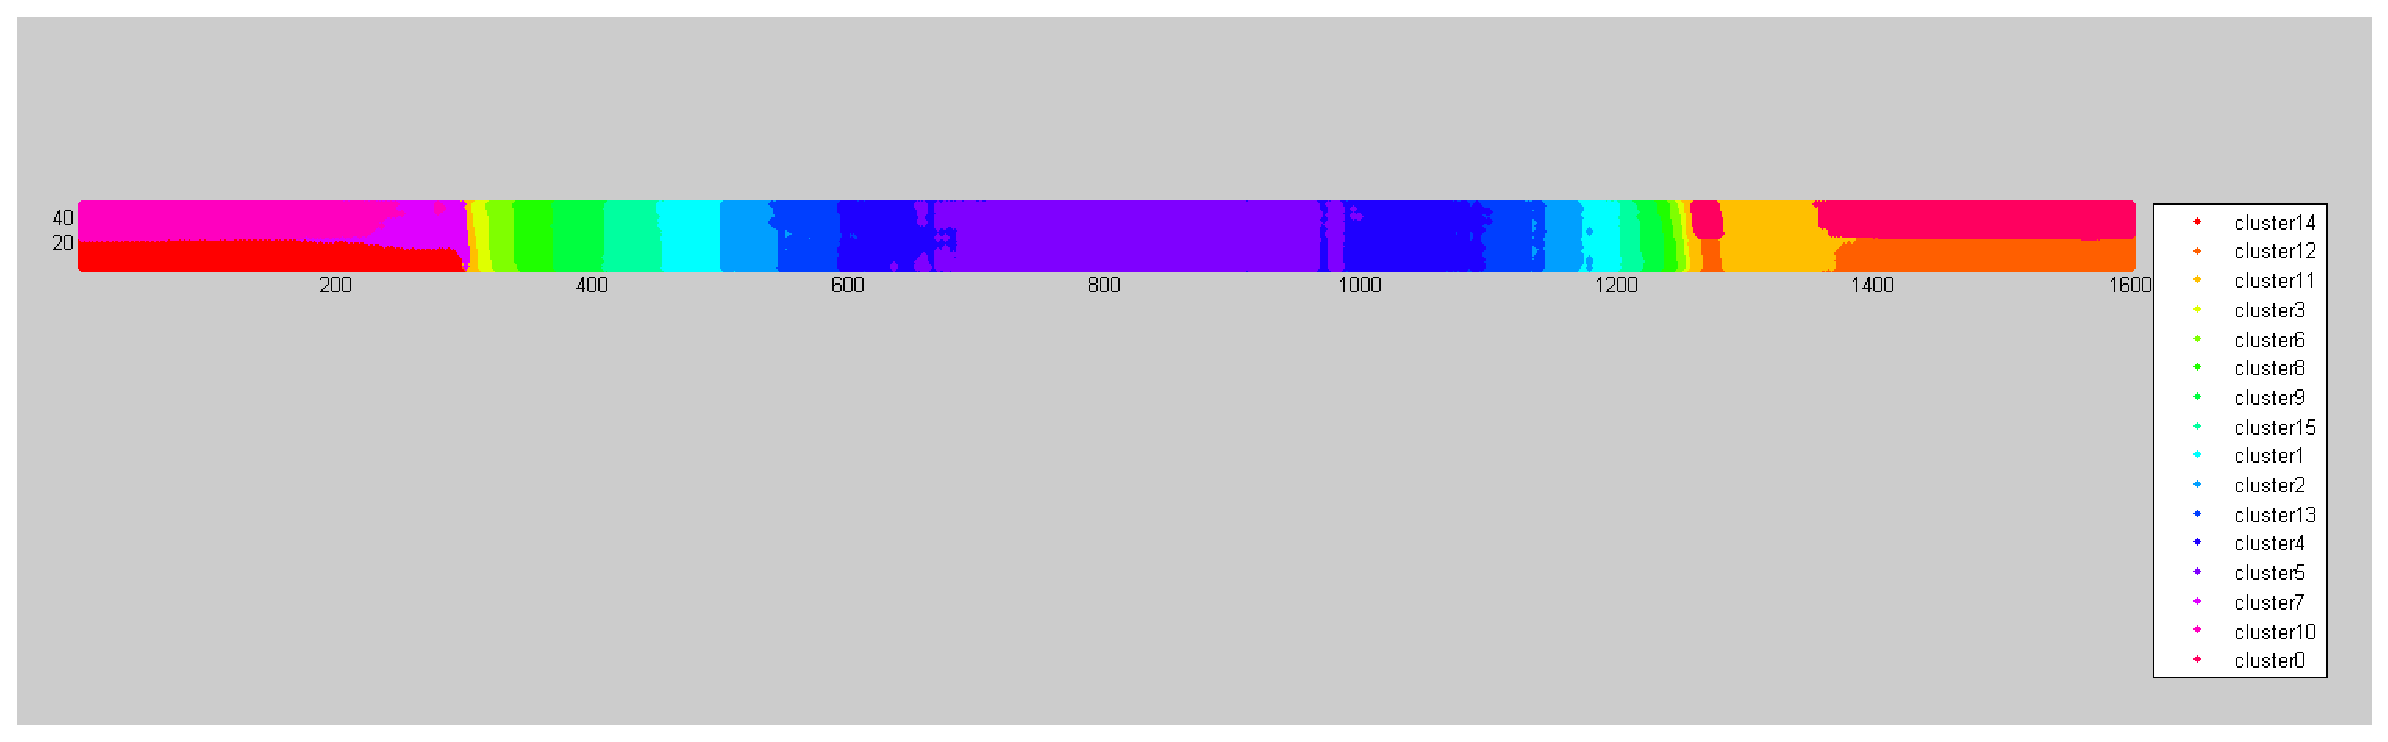
\includegraphics[width=\textwidth]{fig422} 
\caption{
\label{fig422}  % use this to reference in text.
16 classifications of Sample 1.}
\end{figure}

\begin{figure}[H]
\centering
\includegraphics[width=\textwidth]{fig423} 
\caption{
\label{fig423}  % use this to reference in text.
16 classifications of Sample 2.}
\end{figure}

It only takes two steps to get the accuracy of the testing data \cite{Lin2}. The first step is to train your prepared dataset which is the random 9 out of 10 sub-samples. The next step is to test the rest sub-sample. Since the test mode is 10-fold cross-validation, there are total 10 sub-samples can be used as the test dataset. 3 out of 10 sub-samples are chosen as testing data sets in our experiment, and trained with different kernel function which includes the linear kernel, the Gaussian radial basis function (RBF) kernel, the polynomial kernel and the sigmoid kernel. The average running time of training the sub-samples with the linear kernel is about 35 hours, and the average running time of testing the sub-sample with the linear kernel is about 30 minutes. The three accuracies with the linear kernel are 96.8875\%, 96.3188\% and 97.5875\%, so the average accuracy is 96.9313\%. The three accuracies with the Gaussian RBF kernel are 87.6438\%, 87.4563\%, and 88.6688\%, so the average accuracy is 87.9230\%. The three accuracies with the polynomial kernel are 80.0875\%, 79.7313\%, and 80.8625\%, so the average accuracy is 80.2271\%. The three accuracies with the sigmoid kernel are 83.0438\%, 82.8063\%, and 83.6438\%, so the average accuracy is 83.1646\%. Table~\ref{tab2} shows the results of SVM with each kernel function.

\makeatletter
\def\hlinewd#1{%
\noalign{\ifnum0=`}\fi\hrule \@height #1 %
\futurelet\reserved@a\@xhline}
\makeatother

\begin{table}[H]
\centering
\begin{tabular}{| c | c | c | c | c |}
\hline
& Linear & Gaussian RBF & Polynomial & Sigmoid \\ [0.5ex] 
%heading
\hlinewd{2pt}
Average accuracy & 96.9313\% & 87.9230\% & 80.2271\% & 83.1646\% \\ [1ex]
\hline
Average training time (seconds) & 125832.172 & 118834.831 & 111687.569 & 118735.707 \\ [1ex]
\hline
Average testing time (seconds) & 1817.163 & 1446.932 & 1278.743 & 1489.109 \\ [1ex]
\hline
\end{tabular}
\caption{Comparing results of each kernel} 
\label{tab2}
\end{table}


%chapter5
\chapter{Discussion and Conclusions}
This Chapter discusses the findings in previous chapters and suggests the best strategies to do the unsupervised learning of hyperspectral images. Also, the limitations of the study and possible directions for future research are discussed.

\section{Discussion of algorithms}
The vegetation detection algorithm is adapted to the hyperspectral image of mud samples to determine the percentage of significant objects. The percentage of significant objects is easy and quick to get by using this algorithm. Since the three most informative bands are chosen for process, the computation is reduced even for large data sets. However, this can also be the disadvantage of this algorithm if there are more than three bands having the same information. If this happens, the three bands should be randomly chosen from those bands having the same information. 

The k-means algorithm is used for partitioning the hyperspectral image with the pre-defined k. If a dataset is dense and clear, the result of the k-mean algorithm is better. According to the running time in the previous chapter, this algorithm is relatively efficient and scalable for large data sets. The sum of squared error is a very good standard to determine the value of k. Since k is user-defined and must be determined at first, finding out the value of k may take more time than just processing the dataset by the k-means algorithm. Iterations is processed according to the initial clustering, so the computation is costly comparing to the vegetation detection algorithm.

Support vector machine (SVM) is used to train the data and predict another data for better accuracy by using 10-fold cross-validation. SVM can use the three kernel function instead of non-linear mapping, which can save amount of running time. The problem can be treated as finding the optimal solution in SVM, so Non-linear data can be solved by finding the optimal hyper-plane in a high dimensional space. However, since SVM belongs to supervised learning, the dataset must be labelled and the computation is more costly than the k-means algorithm for large data sets.

\section{Conclusions}
Since we determine the percentage of the significant objects by using algorithm for vegetation detection, we have set the bar for the upcoming data mining technique, the k-means algorithm. When we find the groups whose percentage is less than 3.5\%, we definitely need to pay an attention to the groups and find out whether they are what we want. 

Vegetation detection helps us determine the percentage of the significant objects. The percentage is a reference of determining the \begin{math}k\end{math} value. During the process of \begin{math}k=2\end{math} to \begin{math}k=24\end{math} in the k-means algorithm, if the percentage of a cluster is found to be below 3.5%, the corresponding \begin{math}k\end{math} value should be stored as a candidate for further process. It helps us narrow down the selection of the k value.\begin{math}k=16\end{math} meets the requirements of having the least sum of squared errors and stable structure. Therefore, \begin{math}k=16\end{math} is chosen for the k-means algorithm for labeling each pixel in the hyperspectral image. After the dataset is stuffed with cluster label, a supervised learning technique - support venter machine (SVM) will be used for training and testing the dataset with high accuracy. 

10-fold cross validation is used for test mode with 16000 pixels in each fold. Since each pixel has many bands available, each pixel of the mud sample can be considered as a sample and a band as a feature. Therefore, we have 144000 training sample, 811 features each and 16000 test samples. The four kernel functions of support vector machine we used are the linear kernel, the Gaussian radial basis function, the polynomial kernel and sigmoid kernel. The polynomial kernel runs faster than the other three kernels, but the accuracy of the polynomial kernel is the worst. The linear kernel has the best accuracy of all the kernels, but the running time is the worst. The parameters of all the kernels here are default. Therefore, the accuracies of some kernels can be improve by tuning the parameters. That is one of the main reasons why the linear kernel has the best accuracy. However, the main purpose here is not to introduce how the parameters are tuned, but the hybrid system. 

\section{Limitations}
Since we only have two hyperspectral images, the number of samples may not be enough. Therefore, 10-fold cross-validation is used as the test mode. More samples of hyperspectral images will improve the accuracy. The running time is more concerned as this system runs. A 64-bit operating system is a must, and there is no way you can run this kind of large datasets in a 32-bit OS because the minimum heap size of processing the dataset for memory is 6 GB. 

\section{Future Work}
It will be desirable to include in future research some additional models, such as Hierarchical Methods, Bayesian Belief Networks and Probabilistic Model-Based Clustering. Adding more pre-processing or post-processing step is better to improve the accuracy, but more costly. Also, the hyperspectral images can be expanded to include additional factors that may be able to identify the objects with single pixel. The mud sample in this study is just a tool to demonstrate the hybrid system can have a better accuracy. The mud sample can be replaced by any other kinds of hyperspectral images, and even this hybrid system can be extended into other fields required for clustering or classifications. The scatter plot of NIR band and red band from vegetation detection algorithm can be developed with more index value. With more index value available, we can determine more percentage of clusters in order to determine the k value fast.


%references
\newpage
\begin{thebibliography}{100}
\bibitem{Lan2002} Landarebe, D. Hyperspectral image data analysis. \emph{IEEE Signal Processing Magazine}(2002), 17-28.
\bibitem{lili} Li, Z., Li, L., Zhang, R., and Ma, J. An improved classification method for hyperspectral data based on spectral and morphological information. \emph{International Journal of Remote Sensing}(2011), vol.32, 2919-2929.
\bibitem{GVG} Gamps-Valls, G., Tuia, D., Bruzzone, L., and Atli Benediktsson, J. Advances in Hyperspectral Image Classification: Earth monitoring with statistical learning methods. \emph{Signal Processing Magazein, IEEE Journal 
}(2014), 1007-1011.
\bibitem{SC} Starr, C. \emph{Biology: Concepts and Application}, Thomson Brooks/Cole, 2005.
\bibitem{HanJ} Han, J., Kamber, M., and Pei, J. \emph{Data Mining: Concepts and Techniques.}, Morgan Kaufmann Publishers, 2011.
\bibitem{MGLM} Mercier, G., and Lennon, M. Support vector machines for hyperspectral image classification with spectral-based kernels. \emph{Geoscience and Remote Sensing Symposium}(2003), vol.1, 288-290.
\bibitem{Raj} Chouhan, R., and Rao, N. Vegetation Detection in Multi Spectral Remote Sensing Images: Protective Role-analysis of Vegetation in 2004 Indian Ocean Tsunami. PDPM Indian Institute of Information Technology, 2011.
\bibitem{WFH} Witten, I., Frank, E., and Hall, M. \emph{Data Mining: Practical Machine Learning Tools and Techniques}, Morgan Kaufmann Publishers, 2011.
\bibitem{Lin} Chang, C., and Lin, C. LIVSVM: a library for support vector machines. \emph{ACM Transactions on Intelligent Systems and Technology}(2011), vol.2, 1-27.
\bibitem{Lin2} Hsu, C., Chang, C., and Lin, C. A paractical guide to support vector classification. \emph{PDF Online}, May, 2009.
\bibitem{Fehr} Fehr, J., Arreola, K., and Burkhardt, H. Fast Support Vector Machine Classification of Very Large Datasets. \emph{Studies in Classification, Data Analysis, and Knowledge Organization}(2008), 11-18.
\bibitem{McCue} McCue, R. A Comparison of the Accuracy of Support Vector Machine and Naive Bayes Algorithms in Spam Classification, University of California at Santa Cruz, Nov,2009.
\bibitem{NCK} Zhang, B., Li, S., Wu, C., Gao, L., Zhang, W., and Peng, M. A neighbourhood-constrained k-means approach to classify very high spatial resolution hyperspectral imagery. \emph{Remote Sensing Letters}(2013), Vol.4, Issue.2, 161-170.
\bibitem{KJE} Koonsanit, K., Jaruskulchai, C., and Eiumnoh, A. Parameter-Free K-Means Clustering Algorithm for Satellite Imagery Application. \emph{Information Science and Applications (ICISA)}(2012), 1-6.
\bibitem{BAC} Braun, A.C., Weidner, U., and Hinz, S. Support vector machines, import vector machines and relevance vector machines for hyperspectral classification �C A comparison. \emph{Hyperspectral Image and Signal Processing: Evolution in Remote Sensing}(2011), 1-4.
\bibitem{GMGW} Gao, H., Mandal, M.K., Guo, G., and Wan, J. Semisupervised Hyperspectral Image Classification With SVM and PSO. \emph{Measuring Technology and Mechatronics Automation (ICMTMA)}(2010), vol.3, 312-324.

\end{thebibliography}


\end{document}

